\documentclass{article}

% CS 224W milestone: NeurIPS style is fine, no page limit, keep it concise.
\PassOptionsToPackage{numbers,compress}{natbib}
\usepackage[preprint]{neurips_2022}

\usepackage[utf8]{inputenc}
\usepackage[T1]{fontenc}
\usepackage{url}
\usepackage{booktabs}
\usepackage{amsfonts,amsmath,amssymb}
\usepackage{microtype}
\usepackage{xcolor}
\usepackage{graphicx}
\usepackage{enumitem}
\usepackage{listings}
\usepackage{tikz}
\usetikzlibrary{arrows.meta,positioning,calc}
\usepackage{hyperref}
\hypersetup{colorlinks=true,linkcolor=blue!50!black,citecolor=blue!50!black,urlcolor=blue!50!black}
\setlength{\textfloatsep}{9pt}
\setlength{\intextsep}{7pt}
\setlist{nosep,leftmargin=1.2em}

\makeatletter
\renewcommand{\@noticestring}{CS 224W (Fall 2026) project milestone. Project type 1: real-world application of GNNs.}
\makeatother

% every number below is a macro written by scripts/make_numbers_final.py from the per-run results (never typed by hand)
% generated by scripts/make_numbers_final.py -- do not edit
\newcommand{\AgeOldSteps}{200}
\newcommand{\ArchText}{Every memory model leaks after a log-only deletion (LiRA AUC on scores 0.84 for TGN, 0.88 for JODIE, 0.75 for DyRep), while the memory-free control forgets by construction but loses accuracy. DyRep's neighbourhood reads make its cones much larger than TGN's and JODIE's, which read two memories; the contractive cell trades accuracy for a provable error bound.}
\newcommand{\ArrivalRelLastfm}{+2.32}
\newcommand{\ArrivalRelMooc}{+0.13}
\newcommand{\ArrivalRelReddit}{-0.13}
\newcommand{\ArrivalRelReview}{+1.37}
\newcommand{\ArrivalRelWiki}{+0.13}
\newcommand{\ArrivalStdLastfm}{2.8}
\newcommand{\ArrivalStdMooc}{2.8}
\newcommand{\ArrivalStdReddit}{0.1}
\newcommand{\ArrivalStdReview}{4.7}
\newcommand{\ArrivalStdWiki}{0.6}
\newcommand{\AttSpearmanListLastfm}{??}
\newcommand{\AttSpearmanListMooc}{+0.20}
\newcommand{\AttSpearmanListReddit}{+0.19}
\newcommand{\AttSpearmanListReview}{??}
\newcommand{\AttSpearmanListWiki}{+0.27}
\newcommand{\AttTopOneListLastfm}{??}
\newcommand{\AttTopOneListMooc}{26}
\newcommand{\AttTopOneListReddit}{28}
\newcommand{\AttTopOneListReview}{??}
\newcommand{\AttTopOneListWiki}{45}
\newcommand{\AttTopOneTotalHiLastfm}{??}
\newcommand{\AttTopOneTotalHiMooc}{14}
\newcommand{\AttTopOneTotalHiReddit}{24}
\newcommand{\AttTopOneTotalHiReview}{??}
\newcommand{\AttTopOneTotalHiWiki}{20}
\newcommand{\AttTopOneTotalLastfm}{??}
\newcommand{\AttTopOneTotalLoLastfm}{??}
\newcommand{\AttTopOneTotalLoMooc}{7}
\newcommand{\AttTopOneTotalLoReddit}{13}
\newcommand{\AttTopOneTotalLoReview}{??}
\newcommand{\AttTopOneTotalLoWiki}{12}
\newcommand{\AttTopOneTotalMooc}{10}
\newcommand{\AttTopOneTotalReddit}{18}
\newcommand{\AttTopOneTotalReview}{??}
\newcommand{\AttTopOneTotalSeedMaxLastfm}{??}
\newcommand{\AttTopOneTotalSeedMaxMooc}{17}
\newcommand{\AttTopOneTotalSeedMaxReddit}{21}
\newcommand{\AttTopOneTotalSeedMaxReview}{??}
\newcommand{\AttTopOneTotalSeedMaxWiki}{28}
\newcommand{\AttTopOneTotalSeedMinLastfm}{??}
\newcommand{\AttTopOneTotalSeedMinMooc}{4}
\newcommand{\AttTopOneTotalSeedMinReddit}{13}
\newcommand{\AttTopOneTotalSeedMinReview}{??}
\newcommand{\AttTopOneTotalSeedMinWiki}{8}
\newcommand{\AttTopOneTotalWiki}{16}
\newcommand{\BenchAgeAllSpeedEffLastfm}{0.8}
\newcommand{\BenchAgeAllSpeedEffMooc}{0.8}
\newcommand{\BenchAgeAllSpeedEffReddit}{1.0}
\newcommand{\BenchAgeAllSpeedEffWiki}{4.1}
\newcommand{\BenchAgeMidSpeedEffLastfm}{1.7}
\newcommand{\BenchAgeMidSpeedEffMooc}{1.2}
\newcommand{\BenchAgeMidSpeedEffReddit}{7.0}
\newcommand{\BenchAgeMidSpeedEffWiki}{6.2}
\newcommand{\BenchAgeMidSpeedLastfm}{12}
\newcommand{\BenchAgeMidSpeedMooc}{16}
\newcommand{\BenchAgeMidSpeedReddit}{9}
\newcommand{\BenchAgeMidSpeedWiki}{20}
\newcommand{\BenchAgeOldSpeedEffLastfm}{0.8}
\newcommand{\BenchAgeOldSpeedEffMooc}{0.8}
\newcommand{\BenchAgeOldSpeedEffReddit}{0.9}
\newcommand{\BenchAgeOldSpeedEffWiki}{??}
\newcommand{\BenchAgeOldSpeedLastfm}{0.8}
\newcommand{\BenchAgeOldSpeedMooc}{1.0}
\newcommand{\BenchAgeOldSpeedReddit}{0.9}
\newcommand{\BenchAgeOldSpeedReview}{??}
\newcommand{\BenchAgeOldSpeedWiki}{??}
\newcommand{\BenchAgeRecentSpeedEffLastfm}{2.5}
\newcommand{\BenchAgeRecentSpeedEffMooc}{2.6}
\newcommand{\BenchAgeRecentSpeedEffReddit}{6.0}
\newcommand{\BenchAgeRecentSpeedEffWiki}{3.8}
\newcommand{\BenchAgeRecentSpeedLastfm}{6}
\newcommand{\BenchAgeRecentSpeedMooc}{7}
\newcommand{\BenchAgeRecentSpeedReddit}{10}
\newcommand{\BenchAgeRecentSpeedReview}{??}
\newcommand{\BenchAgeRecentSpeedWiki}{8}
\newcommand{\BenchAgeWindowLastfm}{500}
\newcommand{\BenchAgeWindowMooc}{309}
\newcommand{\BenchAgeWindowReddit}{500}
\newcommand{\BenchAgeWindowReview}{??}
\newcommand{\BenchAgeWindowWiki}{119}
\newcommand{\BenchBatchSpeedLastfm}{1.0}
\newcommand{\BenchBatchSpeedMooc}{0.9}
\newcommand{\BenchBatchSpeedReddit}{1.4}
\newcommand{\BenchBatchSpeedReview}{4.4}
\newcommand{\BenchBatchSpeedWiki}{5.1}
\newcommand{\BenchExactMsLastfm}{7.1}
\newcommand{\BenchExactMsMooc}{0.7}
\newcommand{\BenchExactMsReddit}{2.4}
\newcommand{\BenchExactMsReview}{3.0}
\newcommand{\BenchExactMsWiki}{0.8}
\newcommand{\BenchReplayMsLastfm}{29.6}
\newcommand{\BenchReplayMsMooc}{23.9}
\newcommand{\BenchReplayMsReddit}{37.9}
\newcommand{\BenchReplayMsReview}{27.2}
\newcommand{\BenchReplayMsWiki}{30.5}
\newcommand{\BenchSpeedEffLastfm}{1.5}
\newcommand{\BenchSpeedEffMooc}{0.9}
\newcommand{\BenchSpeedEffReddit}{5.9}
\newcommand{\BenchSpeedEffReview}{8.2}
\newcommand{\BenchSpeedEffWiki}{8.4}
\newcommand{\BenchSpeedLastfm}{3}
\newcommand{\BenchSpeedMooc}{18}
\newcommand{\BenchSpeedReddit}{9}
\newcommand{\BenchSpeedReview}{9}
\newcommand{\BenchSpeedWiki}{30}
\newcommand{\BenchStreamArrivalMsLastfm}{0.7}
\newcommand{\BenchStreamArrivalMsMooc}{0.6}
\newcommand{\BenchStreamArrivalMsReddit}{0.8}
\newcommand{\BenchStreamArrivalMsReview}{??}
\newcommand{\BenchStreamArrivalMsWiki}{0.7}
\newcommand{\BenchStreamEpsMsLastfm}{2.3}
\newcommand{\BenchStreamEpsMsMooc}{7.8}
\newcommand{\BenchStreamEpsMsReddit}{9.8}
\newcommand{\BenchStreamEpsMsReview}{??}
\newcommand{\BenchStreamEpsMsWiki}{4.6}
\newcommand{\BenchStreamExactMsLastfm}{2.5}
\newcommand{\BenchStreamExactMsMooc}{13.9}
\newcommand{\BenchStreamExactMsReddit}{12.2}
\newcommand{\BenchStreamExactMsReview}{??}
\newcommand{\BenchStreamExactMsWiki}{4.9}
\newcommand{\BenchStreamReplayMsLastfm}{3.3}
\newcommand{\BenchStreamReplayMsMooc}{12.4}
\newcommand{\BenchStreamReplayMsReddit}{19.0}
\newcommand{\BenchStreamReplayMsReview}{??}
\newcommand{\BenchStreamReplayMsWiki}{9.5}
\newcommand{\BenchStreamWalkMsLastfm}{2.2}
\newcommand{\BenchStreamWalkMsMooc}{10.1}
\newcommand{\BenchStreamWalkMsReddit}{10.8}
\newcommand{\BenchStreamWalkMsReview}{??}
\newcommand{\BenchStreamWalkMsWiki}{5.1}
\newcommand{\BenchWalkSpeedEffLastfm}{1.6}
\newcommand{\BenchWalkSpeedEffMooc}{1.2}
\newcommand{\BenchWalkSpeedEffReddit}{2.5}
\newcommand{\BenchWalkSpeedEffReview}{1.8}
\newcommand{\BenchWalkSpeedEffWiki}{2.4}
\newcommand{\BenchWalkSpeedLastfm}{2.0}
\newcommand{\BenchWalkSpeedMooc}{2.1}
\newcommand{\BenchWalkSpeedReddit}{2.6}
\newcommand{\BenchWalkSpeedReview}{1.8}
\newcommand{\BenchWalkSpeedWiki}{2.6}
\newcommand{\BufOneRelLastfm}{-4.7}
\newcommand{\BufOneRelMooc}{-11.3}
\newcommand{\BufOneRelReddit}{-1.5}
\newcommand{\BufOneRelReview}{??}
\newcommand{\BufOneRelWiki}{-4.9}
\newcommand{\CertEightFive}{99.2}
\newcommand{\CertNineFive}{20.3}
\newcommand{\CertRepairCostEightCell}{0.44}
\newcommand{\CertRepairCostNineCell}{0.45}
\newcommand{\CertRepairCostNineFiveCell}{0.46}
\newcommand{\CertRepairHoldsEightCell}{100}
\newcommand{\CertRepairHoldsNineCell}{100}
\newcommand{\CertRepairHoldsNineFiveCell}{100}
\newcommand{\CertSevenFive}{99.9}
\newcommand{\ConVanillaJown}{1.11}
\newcommand{\ConVanillaJsum}{2.04}
\newcommand{\ConVanillaSumMed}{2.04}
\newcommand{\CrnnMrrLoss}{6.3}
\newcommand{\DelEpsCostLastfm}{0.12}
\newcommand{\DelEpsCostMooc}{0.37}
\newcommand{\DelEpsCostReddit}{0.24}
\newcommand{\DelEpsCostReview}{0.01}
\newcommand{\DelEpsCostWiki}{0.23}
\newcommand{\DelExactCostLastfm}{0.93}
\newcommand{\DelExactCostMooc}{0.95}
\newcommand{\DelExactCostReddit}{0.79}
\newcommand{\DelExactCostReview}{0.37}
\newcommand{\DelExactCostWiki}{0.30}
\newcommand{\DelExactMrrAfterLastfm}{0.079}
\newcommand{\DelExactMrrAfterMooc}{0.150}
\newcommand{\DelExactMrrAfterReddit}{0.729}
\newcommand{\DelExactMrrAfterReview}{0.380}
\newcommand{\DelExactMrrAfterWiki}{0.641}
\newcommand{\DelKhopCostLastfm}{0.93}
\newcommand{\DelKhopCostMooc}{0.95}
\newcommand{\DelKhopCostReddit}{0.72}
\newcommand{\DelKhopCostReview}{0.18}
\newcommand{\DelKhopCostWiki}{0.27}
\newcommand{\DelNoneMrrAfterLastfm}{0.079}
\newcommand{\DelNoneMrrAfterMooc}{0.149}
\newcommand{\DelNoneMrrAfterReddit}{0.728}
\newcommand{\DelNoneMrrAfterReview}{0.381}
\newcommand{\DelNoneMrrAfterWiki}{0.639}
\newcommand{\DelProbeExactLastfm}{0.49}
\newcommand{\DelProbeExactMooc}{0.49}
\newcommand{\DelProbeExactReddit}{0.50}
\newcommand{\DelProbeExactReview}{0.49}
\newcommand{\DelProbeExactWiki}{0.51}
\newcommand{\DelProbeResetLastfm}{0.70}
\newcommand{\DelProbeResetMooc}{0.67}
\newcommand{\DelProbeResetReddit}{0.87}
\newcommand{\DelProbeResetReview}{1.00}
\newcommand{\DelProbeResetWiki}{0.88}
\newcommand{\DelProbeRestartLastfm}{0.70}
\newcommand{\DelProbeRestartMooc}{0.67}
\newcommand{\DelProbeRestartReddit}{0.79}
\newcommand{\DelProbeRestartReview}{1.00}
\newcommand{\DelProbeRestartWiki}{0.78}
\newcommand{\DelProbeStoreLastfm}{0.50}
\newcommand{\DelProbeStoreMooc}{0.50}
\newcommand{\DelProbeStoreReddit}{0.59}
\newcommand{\DelProbeStoreReview}{0.56}
\newcommand{\DelProbeStoreWiki}{0.64}
\newcommand{\DelReplayCostLastfm}{0.97}
\newcommand{\DelReplayCostMooc}{0.97}
\newcommand{\DelReplayCostReddit}{0.97}
\newcommand{\DelReplayCostReview}{1.00}
\newcommand{\DelReplayCostWiki}{0.92}
\newcommand{\DelResetMrrAfterLastfm}{0.135}
\newcommand{\DelResetMrrAfterMooc}{0.122}
\newcommand{\DelResetMrrAfterReddit}{0.656}
\newcommand{\DelResetMrrAfterReview}{0.317}
\newcommand{\DelResetMrrAfterWiki}{0.618}
\newcommand{\DyrepConeLastfm}{??}
\newcommand{\DyrepConeMooc}{90.6}
\newcommand{\DyrepConeRatio}{741}
\newcommand{\DyrepConeReddit}{64.4}
\newcommand{\DyrepConeReview}{??}
\newcommand{\DyrepConeWiki}{14.7}
\newcommand{\DyrepLiraQStoreWiki}{0.75}
\newcommand{\DyrepLiraStoreLastfm}{??}
\newcommand{\DyrepLiraStoreMooc}{0.65}
\newcommand{\DyrepLiraStoreReddit}{0.71}
\newcommand{\DyrepLiraStoreReview}{??}
\newcommand{\DyrepLiraStoreWiki}{0.78}
\newcommand{\DyrepMrrLastfm}{??}
\newcommand{\DyrepMrrMooc}{0.108}
\newcommand{\DyrepMrrReddit}{0.704}
\newcommand{\DyrepMrrReview}{??}
\newcommand{\DyrepMrrWiki}{0.528}
\newcommand{\EpsCostLastfm}{1.08}
\newcommand{\EpsCostMooc}{2.20}
\newcommand{\EpsCostReddit}{1.89}
\newcommand{\EpsCostReview}{1.07}
\newcommand{\EpsCostWiki}{1.24}
\newcommand{\EpsRelLastfm}{+0.09}
\newcommand{\EpsRelMooc}{+0.32}
\newcommand{\EpsRelReddit}{-0.01}
\newcommand{\EpsRelReview}{+0.01}
\newcommand{\EpsRelWiki}{+0.01}
\newcommand{\ExConeEffLastfm}{13.7}
\newcommand{\ExConeEffMooc}{52.2}
\newcommand{\ExConeEffReddit}{0.4}
\newcommand{\ExConeEffReview}{0.0}
\newcommand{\ExConeEffWiki}{0.5}
\newcommand{\ExConeLastfm}{5.78}
\newcommand{\ExConeMooc}{0.05}
\newcommand{\ExConePNinetyLastfm}{63}
\newcommand{\ExConePNinetyMooc}{81}
\newcommand{\ExConePNinetyReddit}{28}
\newcommand{\ExConePNinetyReview}{0}
\newcommand{\ExConePNinetyWiki}{7}
\newcommand{\ExConeReddit}{0.38}
\newcommand{\ExConeReview}{0.02}
\newcommand{\ExConeWiki}{0.02}
\newcommand{\ExDoubleMax}{0}
\newcommand{\ExDoubleTrials}{983}
\newcommand{\ExMax}{1.0e-06}
\newcommand{\ExMaxAll}{1.0e-06}
\newcommand{\ExMaxDyrep}{1.6e-05}
\newcommand{\ExMaxJodie}{2.5e-06}
\newcommand{\ExNoEffectLastfm}{26}
\newcommand{\ExNoEffectMooc}{54}
\newcommand{\ExNoEffectReddit}{11}
\newcommand{\ExNoEffectReview}{6}
\newcommand{\ExNoEffectWiki}{57}
\newcommand{\ExNoPadFail}{20}
\newcommand{\ExTotal}{9,865}
\newcommand{\ExTotalAll}{12,824}
\newcommand{\ExactCostLastfm}{1.11}
\newcommand{\ExactCostMooc}{23.10}
\newcommand{\ExactCostReddit}{13.69}
\newcommand{\ExactCostReview}{1.10}
\newcommand{\ExactCostWiki}{1.30}
\newcommand{\ExactKTwentyFiveMax}{0.60}
\newcommand{\ExactKTwentyFiveMin}{0.44}
\newcommand{\HistJournalGBLastfm}{0.8}
\newcommand{\HistJournalGBMooc}{0.2}
\newcommand{\HistJournalGBReddit}{0.6}
\newcommand{\HistJournalGBReview}{5.3}
\newcommand{\HistJournalGBWiki}{0.1}
\newcommand{\HistPassSecLastfm}{2.41}
\newcommand{\HistPassSecMooc}{0.53}
\newcommand{\HistPassSecReddit}{1.60}
\newcommand{\HistPassSecReview}{??}
\newcommand{\HistPassSecWiki}{0.28}
\newcommand{\InflQueriesLastfm}{??}
\newcommand{\InflQueriesMooc}{100}
\newcommand{\InflQueriesReddit}{62}
\newcommand{\InflQueriesReview}{??}
\newcommand{\InflQueriesWiki}{93}
\newcommand{\JournalMBLastfm}{148}
\newcommand{\JournalMBMooc}{28}
\newcommand{\JournalMBReddit}{103}
\newcommand{\JournalMBReview}{400}
\newcommand{\JournalMBWiki}{14}
\newcommand{\JournalWikiMB}{14}
\newcommand{\LiraAfterFiftyQEpsLastfm}{0.65}
\newcommand{\LiraAfterFiftyQEpsMooc}{0.54}
\newcommand{\LiraAfterFiftyQEpsReddit}{0.63}
\newcommand{\LiraAfterFiftyQEpsReview}{0.86}
\newcommand{\LiraAfterFiftyQEpsWiki}{0.53}
\newcommand{\LiraAfterFiftyQExactLastfm}{0.50}
\newcommand{\LiraAfterFiftyQExactMooc}{0.51}
\newcommand{\LiraAfterFiftyQExactReddit}{0.51}
\newcommand{\LiraAfterFiftyQExactReview}{0.51}
\newcommand{\LiraAfterFiftyQExactWiki}{0.50}
\newcommand{\LiraAfterFiftyQKhopLastfm}{0.51}
\newcommand{\LiraAfterFiftyQKhopMooc}{0.51}
\newcommand{\LiraAfterFiftyQKhopReddit}{0.56}
\newcommand{\LiraAfterFiftyQKhopReview}{0.65}
\newcommand{\LiraAfterFiftyQKhopWiki}{0.56}
\newcommand{\LiraAfterFiftyQResetLastfm}{0.68}
\newcommand{\LiraAfterFiftyQResetMooc}{0.72}
\newcommand{\LiraAfterFiftyQResetReddit}{0.86}
\newcommand{\LiraAfterFiftyQResetReview}{1.00}
\newcommand{\LiraAfterFiftyQResetWiki}{0.82}
\newcommand{\LiraAfterFiftyQRestartLastfm}{0.66}
\newcommand{\LiraAfterFiftyQRestartMooc}{0.69}
\newcommand{\LiraAfterFiftyQRestartReddit}{0.85}
\newcommand{\LiraAfterFiftyQRestartReview}{0.99}
\newcommand{\LiraAfterFiftyQRestartWiki}{0.81}
\newcommand{\LiraAfterFiftyQStoreLastfm}{0.66}
\newcommand{\LiraAfterFiftyQStoreMooc}{0.65}
\newcommand{\LiraAfterFiftyQStoreReddit}{0.87}
\newcommand{\LiraAfterFiftyQStoreReview}{0.97}
\newcommand{\LiraAfterFiftyQStoreWiki}{0.83}
\newcommand{\LiraAfterFiftyWEpsLastfm}{0.63}
\newcommand{\LiraAfterFiftyWEpsMooc}{0.55}
\newcommand{\LiraAfterFiftyWEpsReddit}{0.65}
\newcommand{\LiraAfterFiftyWEpsReview}{0.81}
\newcommand{\LiraAfterFiftyWEpsWiki}{0.55}
\newcommand{\LiraAfterFiftyWExactLastfm}{0.50}
\newcommand{\LiraAfterFiftyWExactMooc}{0.50}
\newcommand{\LiraAfterFiftyWExactReddit}{0.50}
\newcommand{\LiraAfterFiftyWExactReview}{0.50}
\newcommand{\LiraAfterFiftyWExactWiki}{0.49}
\newcommand{\LiraAfterFiftyWKhopLastfm}{0.51}
\newcommand{\LiraAfterFiftyWKhopMooc}{0.50}
\newcommand{\LiraAfterFiftyWKhopReddit}{0.57}
\newcommand{\LiraAfterFiftyWKhopReview}{0.64}
\newcommand{\LiraAfterFiftyWKhopWiki}{0.53}
\newcommand{\LiraAfterFiftyWResetLastfm}{0.66}
\newcommand{\LiraAfterFiftyWResetMooc}{0.73}
\newcommand{\LiraAfterFiftyWResetReddit}{0.87}
\newcommand{\LiraAfterFiftyWResetReview}{1.00}
\newcommand{\LiraAfterFiftyWResetWiki}{0.84}
\newcommand{\LiraAfterFiftyWRestartLastfm}{0.64}
\newcommand{\LiraAfterFiftyWRestartMooc}{0.71}
\newcommand{\LiraAfterFiftyWRestartReddit}{0.87}
\newcommand{\LiraAfterFiftyWRestartReview}{1.00}
\newcommand{\LiraAfterFiftyWRestartWiki}{0.84}
\newcommand{\LiraAfterFiftyWStoreLastfm}{0.63}
\newcommand{\LiraAfterFiftyWStoreMooc}{0.66}
\newcommand{\LiraAfterFiftyWStoreReddit}{0.90}
\newcommand{\LiraAfterFiftyWStoreReview}{0.98}
\newcommand{\LiraAfterFiftyWStoreWiki}{0.86}
\newcommand{\LiraAfterTwentyQEpsLastfm}{0.65}
\newcommand{\LiraAfterTwentyQEpsMooc}{0.54}
\newcommand{\LiraAfterTwentyQEpsReddit}{0.63}
\newcommand{\LiraAfterTwentyQEpsReview}{0.86}
\newcommand{\LiraAfterTwentyQEpsWiki}{0.54}
\newcommand{\LiraAfterTwentyQExactLastfm}{0.50}
\newcommand{\LiraAfterTwentyQExactMooc}{0.50}
\newcommand{\LiraAfterTwentyQExactReddit}{0.51}
\newcommand{\LiraAfterTwentyQExactReview}{0.50}
\newcommand{\LiraAfterTwentyQExactWiki}{0.50}
\newcommand{\LiraAfterTwentyQKhopLastfm}{0.50}
\newcommand{\LiraAfterTwentyQKhopMooc}{0.50}
\newcommand{\LiraAfterTwentyQKhopReddit}{0.57}
\newcommand{\LiraAfterTwentyQKhopReview}{0.65}
\newcommand{\LiraAfterTwentyQKhopWiki}{0.55}
\newcommand{\LiraAfterTwentyQResetLastfm}{0.67}
\newcommand{\LiraAfterTwentyQResetMooc}{0.72}
\newcommand{\LiraAfterTwentyQResetReddit}{0.85}
\newcommand{\LiraAfterTwentyQResetReview}{1.00}
\newcommand{\LiraAfterTwentyQResetWiki}{0.81}
\newcommand{\LiraAfterTwentyQRestartLastfm}{0.67}
\newcommand{\LiraAfterTwentyQRestartMooc}{0.69}
\newcommand{\LiraAfterTwentyQRestartReddit}{0.84}
\newcommand{\LiraAfterTwentyQRestartReview}{0.99}
\newcommand{\LiraAfterTwentyQRestartWiki}{0.81}
\newcommand{\LiraAfterTwentyQStoreLastfm}{0.65}
\newcommand{\LiraAfterTwentyQStoreMooc}{0.65}
\newcommand{\LiraAfterTwentyQStoreReddit}{0.87}
\newcommand{\LiraAfterTwentyQStoreReview}{0.97}
\newcommand{\LiraAfterTwentyQStoreWiki}{0.84}
\newcommand{\LiraAfterTwentyWEpsLastfm}{0.62}
\newcommand{\LiraAfterTwentyWEpsMooc}{0.55}
\newcommand{\LiraAfterTwentyWEpsReddit}{0.65}
\newcommand{\LiraAfterTwentyWEpsReview}{0.81}
\newcommand{\LiraAfterTwentyWEpsWiki}{0.56}
\newcommand{\LiraAfterTwentyWExactLastfm}{0.50}
\newcommand{\LiraAfterTwentyWExactMooc}{0.50}
\newcommand{\LiraAfterTwentyWExactReddit}{0.49}
\newcommand{\LiraAfterTwentyWExactReview}{0.50}
\newcommand{\LiraAfterTwentyWExactWiki}{0.50}
\newcommand{\LiraAfterTwentyWKhopLastfm}{0.50}
\newcommand{\LiraAfterTwentyWKhopMooc}{0.50}
\newcommand{\LiraAfterTwentyWKhopReddit}{0.56}
\newcommand{\LiraAfterTwentyWKhopReview}{0.65}
\newcommand{\LiraAfterTwentyWKhopWiki}{0.54}
\newcommand{\LiraAfterTwentyWResetLastfm}{0.63}
\newcommand{\LiraAfterTwentyWResetMooc}{0.74}
\newcommand{\LiraAfterTwentyWResetReddit}{0.87}
\newcommand{\LiraAfterTwentyWResetReview}{1.00}
\newcommand{\LiraAfterTwentyWResetWiki}{0.85}
\newcommand{\LiraAfterTwentyWRestartLastfm}{0.67}
\newcommand{\LiraAfterTwentyWRestartMooc}{0.71}
\newcommand{\LiraAfterTwentyWRestartReddit}{0.88}
\newcommand{\LiraAfterTwentyWRestartReview}{1.00}
\newcommand{\LiraAfterTwentyWRestartWiki}{0.85}
\newcommand{\LiraAfterTwentyWStoreLastfm}{0.64}
\newcommand{\LiraAfterTwentyWStoreMooc}{0.66}
\newcommand{\LiraAfterTwentyWStoreReddit}{0.90}
\newcommand{\LiraAfterTwentyWStoreReview}{0.98}
\newcommand{\LiraAfterTwentyWStoreWiki}{0.87}
\newcommand{\LiraBestEpsLastfm}{0.65}
\newcommand{\LiraBestEpsMooc}{0.55}
\newcommand{\LiraBestEpsReddit}{0.64}
\newcommand{\LiraBestEpsReview}{0.86}
\newcommand{\LiraBestEpsWiki}{0.58}
\newcommand{\LiraBestExactLastfm}{0.50}
\newcommand{\LiraBestExactMooc}{0.51}
\newcommand{\LiraBestExactReddit}{0.51}
\newcommand{\LiraBestExactReview}{0.50}
\newcommand{\LiraBestExactWiki}{0.50}
\newcommand{\LiraBestKhopLastfm}{0.51}
\newcommand{\LiraBestKhopMooc}{0.51}
\newcommand{\LiraBestKhopReddit}{0.58}
\newcommand{\LiraBestKhopReview}{0.66}
\newcommand{\LiraBestKhopWiki}{0.56}
\newcommand{\LiraBestResetLastfm}{0.69}
\newcommand{\LiraBestResetMooc}{0.75}
\newcommand{\LiraBestResetReddit}{0.83}
\newcommand{\LiraBestResetReview}{1.00}
\newcommand{\LiraBestResetWiki}{0.82}
\newcommand{\LiraBestRestartLastfm}{0.75}
\newcommand{\LiraBestRestartMooc}{0.71}
\newcommand{\LiraBestRestartReddit}{0.90}
\newcommand{\LiraBestRestartReview}{1.00}
\newcommand{\LiraBestRestartWiki}{0.88}
\newcommand{\LiraBestStoreLastfm}{0.63}
\newcommand{\LiraBestStoreMooc}{0.65}
\newcommand{\LiraBestStoreReddit}{0.90}
\newcommand{\LiraBestStoreReview}{0.98}
\newcommand{\LiraBestStoreWiki}{0.87}
\newcommand{\LiraEpsLastfm}{0.62}
\newcommand{\LiraEpsMooc}{0.55}
\newcommand{\LiraEpsReddit}{0.64}
\newcommand{\LiraEpsReview}{0.81}
\newcommand{\LiraEpsWiki}{0.56}
\newcommand{\LiraExactLastfm}{0.50}
\newcommand{\LiraExactMooc}{0.51}
\newcommand{\LiraExactReddit}{0.51}
\newcommand{\LiraExactReview}{0.50}
\newcommand{\LiraExactWiki}{0.50}
\newcommand{\LiraKHundredQEpsLastfm}{0.86}
\newcommand{\LiraKHundredQEpsMooc}{0.66}
\newcommand{\LiraKHundredQEpsReddit}{0.83}
\newcommand{\LiraKHundredQEpsReview}{??}
\newcommand{\LiraKHundredQEpsWiki}{0.64}
\newcommand{\LiraKHundredQExactLastfm}{0.50}
\newcommand{\LiraKHundredQExactMooc}{0.52}
\newcommand{\LiraKHundredQExactReddit}{0.46}
\newcommand{\LiraKHundredQExactReview}{??}
\newcommand{\LiraKHundredQExactWiki}{0.50}
\newcommand{\LiraKHundredQKhopLastfm}{0.54}
\newcommand{\LiraKHundredQKhopMooc}{0.52}
\newcommand{\LiraKHundredQKhopReddit}{0.71}
\newcommand{\LiraKHundredQKhopReview}{??}
\newcommand{\LiraKHundredQKhopWiki}{0.63}
\newcommand{\LiraKHundredQResetLastfm}{0.94}
\newcommand{\LiraKHundredQResetMooc}{0.97}
\newcommand{\LiraKHundredQResetReddit}{0.95}
\newcommand{\LiraKHundredQResetReview}{??}
\newcommand{\LiraKHundredQResetWiki}{0.89}
\newcommand{\LiraKHundredQRestartLastfm}{0.94}
\newcommand{\LiraKHundredQRestartMooc}{0.94}
\newcommand{\LiraKHundredQRestartReddit}{0.98}
\newcommand{\LiraKHundredQRestartReview}{??}
\newcommand{\LiraKHundredQRestartWiki}{0.92}
\newcommand{\LiraKHundredQStoreLastfm}{0.85}
\newcommand{\LiraKHundredQStoreMooc}{0.75}
\newcommand{\LiraKHundredQStoreReddit}{0.97}
\newcommand{\LiraKHundredQStoreReview}{??}
\newcommand{\LiraKHundredQStoreWiki}{0.92}
\newcommand{\LiraKHundredWEpsLastfm}{0.82}
\newcommand{\LiraKHundredWEpsMooc}{0.68}
\newcommand{\LiraKHundredWEpsReddit}{0.82}
\newcommand{\LiraKHundredWEpsReview}{??}
\newcommand{\LiraKHundredWEpsWiki}{0.59}
\newcommand{\LiraKHundredWExactLastfm}{0.50}
\newcommand{\LiraKHundredWExactMooc}{0.53}
\newcommand{\LiraKHundredWExactReddit}{0.49}
\newcommand{\LiraKHundredWExactReview}{??}
\newcommand{\LiraKHundredWExactWiki}{0.50}
\newcommand{\LiraKHundredWKhopLastfm}{0.51}
\newcommand{\LiraKHundredWKhopMooc}{0.49}
\newcommand{\LiraKHundredWKhopReddit}{0.74}
\newcommand{\LiraKHundredWKhopReview}{??}
\newcommand{\LiraKHundredWKhopWiki}{0.60}
\newcommand{\LiraKHundredWResetLastfm}{0.87}
\newcommand{\LiraKHundredWResetMooc}{0.68}
\newcommand{\LiraKHundredWResetReddit}{0.93}
\newcommand{\LiraKHundredWResetReview}{??}
\newcommand{\LiraKHundredWResetWiki}{0.85}
\newcommand{\LiraKHundredWRestartLastfm}{0.99}
\newcommand{\LiraKHundredWRestartMooc}{0.96}
\newcommand{\LiraKHundredWRestartReddit}{0.99}
\newcommand{\LiraKHundredWRestartReview}{??}
\newcommand{\LiraKHundredWRestartWiki}{0.96}
\newcommand{\LiraKHundredWStoreLastfm}{0.83}
\newcommand{\LiraKHundredWStoreMooc}{0.78}
\newcommand{\LiraKHundredWStoreReddit}{0.98}
\newcommand{\LiraKHundredWStoreReview}{??}
\newcommand{\LiraKHundredWStoreWiki}{0.95}
\newcommand{\LiraKTwentyFiveQEpsLastfm}{0.91}
\newcommand{\LiraKTwentyFiveQEpsMooc}{0.76}
\newcommand{\LiraKTwentyFiveQEpsReddit}{0.94}
\newcommand{\LiraKTwentyFiveQEpsReview}{??}
\newcommand{\LiraKTwentyFiveQEpsWiki}{0.73}
\newcommand{\LiraKTwentyFiveQExactLastfm}{0.54}
\newcommand{\LiraKTwentyFiveQExactMooc}{0.46}
\newcommand{\LiraKTwentyFiveQExactReddit}{0.46}
\newcommand{\LiraKTwentyFiveQExactReview}{??}
\newcommand{\LiraKTwentyFiveQExactWiki}{0.50}
\newcommand{\LiraKTwentyFiveQKhopLastfm}{0.72}
\newcommand{\LiraKTwentyFiveQKhopMooc}{0.63}
\newcommand{\LiraKTwentyFiveQKhopReddit}{0.76}
\newcommand{\LiraKTwentyFiveQKhopReview}{??}
\newcommand{\LiraKTwentyFiveQKhopWiki}{0.70}
\newcommand{\LiraKTwentyFiveQResetLastfm}{0.99}
\newcommand{\LiraKTwentyFiveQResetMooc}{1.00}
\newcommand{\LiraKTwentyFiveQResetReddit}{0.98}
\newcommand{\LiraKTwentyFiveQResetReview}{??}
\newcommand{\LiraKTwentyFiveQResetWiki}{0.95}
\newcommand{\LiraKTwentyFiveQRestartLastfm}{0.98}
\newcommand{\LiraKTwentyFiveQRestartMooc}{0.98}
\newcommand{\LiraKTwentyFiveQRestartReddit}{0.99}
\newcommand{\LiraKTwentyFiveQRestartReview}{??}
\newcommand{\LiraKTwentyFiveQRestartWiki}{0.98}
\newcommand{\LiraKTwentyFiveQStoreLastfm}{0.91}
\newcommand{\LiraKTwentyFiveQStoreMooc}{0.84}
\newcommand{\LiraKTwentyFiveQStoreReddit}{0.98}
\newcommand{\LiraKTwentyFiveQStoreReview}{??}
\newcommand{\LiraKTwentyFiveQStoreWiki}{0.97}
\newcommand{\LiraKTwentyFiveWEpsLastfm}{0.92}
\newcommand{\LiraKTwentyFiveWEpsMooc}{0.71}
\newcommand{\LiraKTwentyFiveWEpsReddit}{0.87}
\newcommand{\LiraKTwentyFiveWEpsReview}{??}
\newcommand{\LiraKTwentyFiveWEpsWiki}{0.74}
\newcommand{\LiraKTwentyFiveWExactLastfm}{0.53}
\newcommand{\LiraKTwentyFiveWExactMooc}{0.52}
\newcommand{\LiraKTwentyFiveWExactReddit}{0.44}
\newcommand{\LiraKTwentyFiveWExactReview}{??}
\newcommand{\LiraKTwentyFiveWExactWiki}{0.51}
\newcommand{\LiraKTwentyFiveWKhopLastfm}{0.60}
\newcommand{\LiraKTwentyFiveWKhopMooc}{0.60}
\newcommand{\LiraKTwentyFiveWKhopReddit}{0.78}
\newcommand{\LiraKTwentyFiveWKhopReview}{??}
\newcommand{\LiraKTwentyFiveWKhopWiki}{0.69}
\newcommand{\LiraKTwentyFiveWResetLastfm}{0.97}
\newcommand{\LiraKTwentyFiveWResetMooc}{0.90}
\newcommand{\LiraKTwentyFiveWResetReddit}{0.98}
\newcommand{\LiraKTwentyFiveWResetReview}{??}
\newcommand{\LiraKTwentyFiveWResetWiki}{0.95}
\newcommand{\LiraKTwentyFiveWRestartLastfm}{0.99}
\newcommand{\LiraKTwentyFiveWRestartMooc}{0.99}
\newcommand{\LiraKTwentyFiveWRestartReddit}{1.00}
\newcommand{\LiraKTwentyFiveWRestartReview}{??}
\newcommand{\LiraKTwentyFiveWRestartWiki}{1.00}
\newcommand{\LiraKTwentyFiveWStoreLastfm}{0.93}
\newcommand{\LiraKTwentyFiveWStoreMooc}{0.85}
\newcommand{\LiraKTwentyFiveWStoreReddit}{0.98}
\newcommand{\LiraKTwentyFiveWStoreReview}{??}
\newcommand{\LiraKTwentyFiveWStoreWiki}{0.98}
\newcommand{\LiraKnowHalfEpsLastfm}{0.51}
\newcommand{\LiraKnowHalfEpsMooc}{0.51}
\newcommand{\LiraKnowHalfEpsReddit}{0.52}
\newcommand{\LiraKnowHalfEpsReview}{0.51}
\newcommand{\LiraKnowHalfEpsWiki}{0.50}
\newcommand{\LiraKnowHalfExactLastfm}{0.50}
\newcommand{\LiraKnowHalfExactMooc}{0.50}
\newcommand{\LiraKnowHalfExactReddit}{0.51}
\newcommand{\LiraKnowHalfExactReview}{0.50}
\newcommand{\LiraKnowHalfExactWiki}{0.50}
\newcommand{\LiraKnowHalfKTwentyFiveQEpsLastfm}{??}
\newcommand{\LiraKnowHalfKTwentyFiveQEpsMooc}{??}
\newcommand{\LiraKnowHalfKTwentyFiveQEpsReddit}{0.49}
\newcommand{\LiraKnowHalfKTwentyFiveQEpsReview}{??}
\newcommand{\LiraKnowHalfKTwentyFiveQEpsWiki}{0.49}
\newcommand{\LiraKnowHalfKTwentyFiveQExactLastfm}{??}
\newcommand{\LiraKnowHalfKTwentyFiveQExactMooc}{??}
\newcommand{\LiraKnowHalfKTwentyFiveQExactReddit}{0.51}
\newcommand{\LiraKnowHalfKTwentyFiveQExactReview}{??}
\newcommand{\LiraKnowHalfKTwentyFiveQExactWiki}{0.50}
\newcommand{\LiraKnowHalfKTwentyFiveQKhopLastfm}{??}
\newcommand{\LiraKnowHalfKTwentyFiveQKhopMooc}{??}
\newcommand{\LiraKnowHalfKTwentyFiveQKhopReddit}{0.50}
\newcommand{\LiraKnowHalfKTwentyFiveQKhopReview}{??}
\newcommand{\LiraKnowHalfKTwentyFiveQKhopWiki}{0.47}
\newcommand{\LiraKnowHalfKTwentyFiveQResetLastfm}{??}
\newcommand{\LiraKnowHalfKTwentyFiveQResetMooc}{??}
\newcommand{\LiraKnowHalfKTwentyFiveQResetReddit}{0.91}
\newcommand{\LiraKnowHalfKTwentyFiveQResetReview}{??}
\newcommand{\LiraKnowHalfKTwentyFiveQResetWiki}{0.78}
\newcommand{\LiraKnowHalfKTwentyFiveQRestartLastfm}{??}
\newcommand{\LiraKnowHalfKTwentyFiveQRestartMooc}{??}
\newcommand{\LiraKnowHalfKTwentyFiveQRestartReddit}{0.55}
\newcommand{\LiraKnowHalfKTwentyFiveQRestartReview}{??}
\newcommand{\LiraKnowHalfKTwentyFiveQRestartWiki}{0.63}
\newcommand{\LiraKnowHalfKTwentyFiveQStoreLastfm}{??}
\newcommand{\LiraKnowHalfKTwentyFiveQStoreMooc}{??}
\newcommand{\LiraKnowHalfKTwentyFiveQStoreReddit}{0.61}
\newcommand{\LiraKnowHalfKTwentyFiveQStoreReview}{??}
\newcommand{\LiraKnowHalfKTwentyFiveQStoreWiki}{0.67}
\newcommand{\LiraKnowHalfKTwentyFiveWEpsLastfm}{??}
\newcommand{\LiraKnowHalfKTwentyFiveWEpsMooc}{??}
\newcommand{\LiraKnowHalfKTwentyFiveWEpsReddit}{0.49}
\newcommand{\LiraKnowHalfKTwentyFiveWEpsReview}{??}
\newcommand{\LiraKnowHalfKTwentyFiveWEpsWiki}{0.49}
\newcommand{\LiraKnowHalfKTwentyFiveWExactLastfm}{??}
\newcommand{\LiraKnowHalfKTwentyFiveWExactMooc}{??}
\newcommand{\LiraKnowHalfKTwentyFiveWExactReddit}{0.60}
\newcommand{\LiraKnowHalfKTwentyFiveWExactReview}{??}
\newcommand{\LiraKnowHalfKTwentyFiveWExactWiki}{0.50}
\newcommand{\LiraKnowHalfKTwentyFiveWKhopLastfm}{??}
\newcommand{\LiraKnowHalfKTwentyFiveWKhopMooc}{??}
\newcommand{\LiraKnowHalfKTwentyFiveWKhopReddit}{0.55}
\newcommand{\LiraKnowHalfKTwentyFiveWKhopReview}{??}
\newcommand{\LiraKnowHalfKTwentyFiveWKhopWiki}{0.60}
\newcommand{\LiraKnowHalfKTwentyFiveWResetLastfm}{??}
\newcommand{\LiraKnowHalfKTwentyFiveWResetMooc}{??}
\newcommand{\LiraKnowHalfKTwentyFiveWResetReddit}{0.97}
\newcommand{\LiraKnowHalfKTwentyFiveWResetReview}{??}
\newcommand{\LiraKnowHalfKTwentyFiveWResetWiki}{0.96}
\newcommand{\LiraKnowHalfKTwentyFiveWRestartLastfm}{??}
\newcommand{\LiraKnowHalfKTwentyFiveWRestartMooc}{??}
\newcommand{\LiraKnowHalfKTwentyFiveWRestartReddit}{0.71}
\newcommand{\LiraKnowHalfKTwentyFiveWRestartReview}{??}
\newcommand{\LiraKnowHalfKTwentyFiveWRestartWiki}{0.84}
\newcommand{\LiraKnowHalfKTwentyFiveWStoreLastfm}{??}
\newcommand{\LiraKnowHalfKTwentyFiveWStoreMooc}{??}
\newcommand{\LiraKnowHalfKTwentyFiveWStoreReddit}{0.75}
\newcommand{\LiraKnowHalfKTwentyFiveWStoreReview}{??}
\newcommand{\LiraKnowHalfKTwentyFiveWStoreWiki}{0.80}
\newcommand{\LiraKnowHalfKhopLastfm}{0.50}
\newcommand{\LiraKnowHalfKhopMooc}{0.50}
\newcommand{\LiraKnowHalfKhopReddit}{0.51}
\newcommand{\LiraKnowHalfKhopReview}{0.50}
\newcommand{\LiraKnowHalfKhopWiki}{0.50}
\newcommand{\LiraKnowHalfQEpsLastfm}{0.51}
\newcommand{\LiraKnowHalfQEpsMooc}{0.49}
\newcommand{\LiraKnowHalfQEpsReddit}{0.52}
\newcommand{\LiraKnowHalfQEpsReview}{0.51}
\newcommand{\LiraKnowHalfQEpsWiki}{0.50}
\newcommand{\LiraKnowHalfQExactLastfm}{0.50}
\newcommand{\LiraKnowHalfQExactMooc}{0.49}
\newcommand{\LiraKnowHalfQExactReddit}{0.51}
\newcommand{\LiraKnowHalfQExactReview}{0.50}
\newcommand{\LiraKnowHalfQExactWiki}{0.50}
\newcommand{\LiraKnowHalfQKhopLastfm}{0.50}
\newcommand{\LiraKnowHalfQKhopMooc}{0.49}
\newcommand{\LiraKnowHalfQKhopReddit}{0.51}
\newcommand{\LiraKnowHalfQKhopReview}{0.49}
\newcommand{\LiraKnowHalfQKhopWiki}{0.50}
\newcommand{\LiraKnowHalfQResetLastfm}{0.66}
\newcommand{\LiraKnowHalfQResetMooc}{0.73}
\newcommand{\LiraKnowHalfQResetReddit}{0.77}
\newcommand{\LiraKnowHalfQResetReview}{0.97}
\newcommand{\LiraKnowHalfQResetWiki}{0.74}
\newcommand{\LiraKnowHalfQRestartLastfm}{0.53}
\newcommand{\LiraKnowHalfQRestartMooc}{0.54}
\newcommand{\LiraKnowHalfQRestartReddit}{0.56}
\newcommand{\LiraKnowHalfQRestartReview}{0.62}
\newcommand{\LiraKnowHalfQRestartWiki}{0.63}
\newcommand{\LiraKnowHalfQStoreLastfm}{0.51}
\newcommand{\LiraKnowHalfQStoreMooc}{0.53}
\newcommand{\LiraKnowHalfQStoreReddit}{0.65}
\newcommand{\LiraKnowHalfQStoreReview}{0.57}
\newcommand{\LiraKnowHalfQStoreWiki}{0.70}
\newcommand{\LiraKnowHalfResetLastfm}{0.66}
\newcommand{\LiraKnowHalfResetMooc}{0.73}
\newcommand{\LiraKnowHalfResetReddit}{0.77}
\newcommand{\LiraKnowHalfResetReview}{0.98}
\newcommand{\LiraKnowHalfResetWiki}{0.74}
\newcommand{\LiraKnowHalfRestartLastfm}{0.66}
\newcommand{\LiraKnowHalfRestartMooc}{0.56}
\newcommand{\LiraKnowHalfRestartReddit}{0.68}
\newcommand{\LiraKnowHalfRestartReview}{0.73}
\newcommand{\LiraKnowHalfRestartWiki}{0.77}
\newcommand{\LiraKnowHalfStoreLastfm}{0.51}
\newcommand{\LiraKnowHalfStoreMooc}{0.55}
\newcommand{\LiraKnowHalfStoreReddit}{0.73}
\newcommand{\LiraKnowHalfStoreReview}{0.62}
\newcommand{\LiraKnowHalfStoreWiki}{0.80}
\newcommand{\LiraKnowHalfWEpsLastfm}{0.50}
\newcommand{\LiraKnowHalfWEpsMooc}{0.51}
\newcommand{\LiraKnowHalfWEpsReddit}{0.50}
\newcommand{\LiraKnowHalfWEpsReview}{0.49}
\newcommand{\LiraKnowHalfWEpsWiki}{0.49}
\newcommand{\LiraKnowHalfWExactLastfm}{0.50}
\newcommand{\LiraKnowHalfWExactMooc}{0.50}
\newcommand{\LiraKnowHalfWExactReddit}{0.50}
\newcommand{\LiraKnowHalfWExactReview}{0.50}
\newcommand{\LiraKnowHalfWExactWiki}{0.50}
\newcommand{\LiraKnowHalfWKhopLastfm}{0.50}
\newcommand{\LiraKnowHalfWKhopMooc}{0.50}
\newcommand{\LiraKnowHalfWKhopReddit}{0.51}
\newcommand{\LiraKnowHalfWKhopReview}{0.50}
\newcommand{\LiraKnowHalfWKhopWiki}{0.49}
\newcommand{\LiraKnowHalfWResetLastfm}{0.54}
\newcommand{\LiraKnowHalfWResetMooc}{0.50}
\newcommand{\LiraKnowHalfWResetReddit}{0.63}
\newcommand{\LiraKnowHalfWResetReview}{0.98}
\newcommand{\LiraKnowHalfWResetWiki}{0.68}
\newcommand{\LiraKnowHalfWRestartLastfm}{0.66}
\newcommand{\LiraKnowHalfWRestartMooc}{0.56}
\newcommand{\LiraKnowHalfWRestartReddit}{0.68}
\newcommand{\LiraKnowHalfWRestartReview}{0.73}
\newcommand{\LiraKnowHalfWRestartWiki}{0.77}
\newcommand{\LiraKnowHalfWStoreLastfm}{0.51}
\newcommand{\LiraKnowHalfWStoreMooc}{0.55}
\newcommand{\LiraKnowHalfWStoreReddit}{0.73}
\newcommand{\LiraKnowHalfWStoreReview}{0.62}
\newcommand{\LiraKnowHalfWStoreWiki}{0.80}
\newcommand{\LiraKnowNoneEpsLastfm}{0.50}
\newcommand{\LiraKnowNoneEpsMooc}{0.50}
\newcommand{\LiraKnowNoneEpsReddit}{0.50}
\newcommand{\LiraKnowNoneEpsReview}{0.50}
\newcommand{\LiraKnowNoneEpsWiki}{0.50}
\newcommand{\LiraKnowNoneExactLastfm}{0.50}
\newcommand{\LiraKnowNoneExactMooc}{0.50}
\newcommand{\LiraKnowNoneExactReddit}{0.50}
\newcommand{\LiraKnowNoneExactReview}{0.50}
\newcommand{\LiraKnowNoneExactWiki}{0.50}
\newcommand{\LiraKnowNoneKTwentyFiveQEpsLastfm}{??}
\newcommand{\LiraKnowNoneKTwentyFiveQEpsMooc}{??}
\newcommand{\LiraKnowNoneKTwentyFiveQEpsReddit}{0.50}
\newcommand{\LiraKnowNoneKTwentyFiveQEpsReview}{??}
\newcommand{\LiraKnowNoneKTwentyFiveQEpsWiki}{0.50}
\newcommand{\LiraKnowNoneKTwentyFiveQExactLastfm}{??}
\newcommand{\LiraKnowNoneKTwentyFiveQExactMooc}{??}
\newcommand{\LiraKnowNoneKTwentyFiveQExactReddit}{0.50}
\newcommand{\LiraKnowNoneKTwentyFiveQExactReview}{??}
\newcommand{\LiraKnowNoneKTwentyFiveQExactWiki}{0.50}
\newcommand{\LiraKnowNoneKTwentyFiveQKhopLastfm}{??}
\newcommand{\LiraKnowNoneKTwentyFiveQKhopMooc}{??}
\newcommand{\LiraKnowNoneKTwentyFiveQKhopReddit}{0.50}
\newcommand{\LiraKnowNoneKTwentyFiveQKhopReview}{??}
\newcommand{\LiraKnowNoneKTwentyFiveQKhopWiki}{0.50}
\newcommand{\LiraKnowNoneKTwentyFiveQResetLastfm}{??}
\newcommand{\LiraKnowNoneKTwentyFiveQResetMooc}{??}
\newcommand{\LiraKnowNoneKTwentyFiveQResetReddit}{0.80}
\newcommand{\LiraKnowNoneKTwentyFiveQResetReview}{??}
\newcommand{\LiraKnowNoneKTwentyFiveQResetWiki}{0.65}
\newcommand{\LiraKnowNoneKTwentyFiveQRestartLastfm}{??}
\newcommand{\LiraKnowNoneKTwentyFiveQRestartMooc}{??}
\newcommand{\LiraKnowNoneKTwentyFiveQRestartReddit}{0.47}
\newcommand{\LiraKnowNoneKTwentyFiveQRestartReview}{??}
\newcommand{\LiraKnowNoneKTwentyFiveQRestartWiki}{0.51}
\newcommand{\LiraKnowNoneKTwentyFiveQStoreLastfm}{??}
\newcommand{\LiraKnowNoneKTwentyFiveQStoreMooc}{??}
\newcommand{\LiraKnowNoneKTwentyFiveQStoreReddit}{0.59}
\newcommand{\LiraKnowNoneKTwentyFiveQStoreReview}{??}
\newcommand{\LiraKnowNoneKTwentyFiveQStoreWiki}{0.63}
\newcommand{\LiraKnowNoneKTwentyFiveWEpsLastfm}{??}
\newcommand{\LiraKnowNoneKTwentyFiveWEpsMooc}{??}
\newcommand{\LiraKnowNoneKTwentyFiveWEpsReddit}{0.50}
\newcommand{\LiraKnowNoneKTwentyFiveWEpsReview}{??}
\newcommand{\LiraKnowNoneKTwentyFiveWEpsWiki}{0.50}
\newcommand{\LiraKnowNoneKTwentyFiveWExactLastfm}{??}
\newcommand{\LiraKnowNoneKTwentyFiveWExactMooc}{??}
\newcommand{\LiraKnowNoneKTwentyFiveWExactReddit}{0.50}
\newcommand{\LiraKnowNoneKTwentyFiveWExactReview}{??}
\newcommand{\LiraKnowNoneKTwentyFiveWExactWiki}{0.50}
\newcommand{\LiraKnowNoneKTwentyFiveWKhopLastfm}{??}
\newcommand{\LiraKnowNoneKTwentyFiveWKhopMooc}{??}
\newcommand{\LiraKnowNoneKTwentyFiveWKhopReddit}{0.50}
\newcommand{\LiraKnowNoneKTwentyFiveWKhopReview}{??}
\newcommand{\LiraKnowNoneKTwentyFiveWKhopWiki}{0.50}
\newcommand{\LiraKnowNoneKTwentyFiveWResetLastfm}{??}
\newcommand{\LiraKnowNoneKTwentyFiveWResetMooc}{??}
\newcommand{\LiraKnowNoneKTwentyFiveWResetReddit}{0.97}
\newcommand{\LiraKnowNoneKTwentyFiveWResetReview}{??}
\newcommand{\LiraKnowNoneKTwentyFiveWResetWiki}{0.95}
\newcommand{\LiraKnowNoneKTwentyFiveWRestartLastfm}{??}
\newcommand{\LiraKnowNoneKTwentyFiveWRestartMooc}{??}
\newcommand{\LiraKnowNoneKTwentyFiveWRestartReddit}{0.63}
\newcommand{\LiraKnowNoneKTwentyFiveWRestartReview}{??}
\newcommand{\LiraKnowNoneKTwentyFiveWRestartWiki}{0.68}
\newcommand{\LiraKnowNoneKTwentyFiveWStoreLastfm}{??}
\newcommand{\LiraKnowNoneKTwentyFiveWStoreMooc}{??}
\newcommand{\LiraKnowNoneKTwentyFiveWStoreReddit}{0.73}
\newcommand{\LiraKnowNoneKTwentyFiveWStoreReview}{??}
\newcommand{\LiraKnowNoneKTwentyFiveWStoreWiki}{0.72}
\newcommand{\LiraKnowNoneKhopLastfm}{0.50}
\newcommand{\LiraKnowNoneKhopMooc}{0.50}
\newcommand{\LiraKnowNoneKhopReddit}{0.50}
\newcommand{\LiraKnowNoneKhopReview}{0.50}
\newcommand{\LiraKnowNoneKhopWiki}{0.50}
\newcommand{\LiraKnowNoneQEpsLastfm}{0.50}
\newcommand{\LiraKnowNoneQEpsMooc}{0.50}
\newcommand{\LiraKnowNoneQEpsReddit}{0.50}
\newcommand{\LiraKnowNoneQEpsReview}{0.50}
\newcommand{\LiraKnowNoneQEpsWiki}{0.50}
\newcommand{\LiraKnowNoneQExactLastfm}{0.50}
\newcommand{\LiraKnowNoneQExactMooc}{0.50}
\newcommand{\LiraKnowNoneQExactReddit}{0.50}
\newcommand{\LiraKnowNoneQExactReview}{0.50}
\newcommand{\LiraKnowNoneQExactWiki}{0.50}
\newcommand{\LiraKnowNoneQKhopLastfm}{0.50}
\newcommand{\LiraKnowNoneQKhopMooc}{0.50}
\newcommand{\LiraKnowNoneQKhopReddit}{0.50}
\newcommand{\LiraKnowNoneQKhopReview}{0.50}
\newcommand{\LiraKnowNoneQKhopWiki}{0.50}
\newcommand{\LiraKnowNoneQResetLastfm}{0.63}
\newcommand{\LiraKnowNoneQResetMooc}{0.70}
\newcommand{\LiraKnowNoneQResetReddit}{0.73}
\newcommand{\LiraKnowNoneQResetReview}{0.97}
\newcommand{\LiraKnowNoneQResetWiki}{0.63}
\newcommand{\LiraKnowNoneQRestartLastfm}{0.52}
\newcommand{\LiraKnowNoneQRestartMooc}{0.51}
\newcommand{\LiraKnowNoneQRestartReddit}{0.53}
\newcommand{\LiraKnowNoneQRestartReview}{0.53}
\newcommand{\LiraKnowNoneQRestartWiki}{0.57}
\newcommand{\LiraKnowNoneQStoreLastfm}{0.52}
\newcommand{\LiraKnowNoneQStoreMooc}{0.50}
\newcommand{\LiraKnowNoneQStoreReddit}{0.59}
\newcommand{\LiraKnowNoneQStoreReview}{0.52}
\newcommand{\LiraKnowNoneQStoreWiki}{0.63}
\newcommand{\LiraKnowNoneResetLastfm}{0.63}
\newcommand{\LiraKnowNoneResetMooc}{0.70}
\newcommand{\LiraKnowNoneResetReddit}{0.73}
\newcommand{\LiraKnowNoneResetReview}{0.98}
\newcommand{\LiraKnowNoneResetWiki}{0.68}
\newcommand{\LiraKnowNoneRestartLastfm}{0.58}
\newcommand{\LiraKnowNoneRestartMooc}{0.51}
\newcommand{\LiraKnowNoneRestartReddit}{0.62}
\newcommand{\LiraKnowNoneRestartReview}{0.62}
\newcommand{\LiraKnowNoneRestartWiki}{0.68}
\newcommand{\LiraKnowNoneStoreLastfm}{0.52}
\newcommand{\LiraKnowNoneStoreMooc}{0.50}
\newcommand{\LiraKnowNoneStoreReddit}{0.65}
\newcommand{\LiraKnowNoneStoreReview}{0.52}
\newcommand{\LiraKnowNoneStoreWiki}{0.73}
\newcommand{\LiraKnowNoneWEpsLastfm}{0.50}
\newcommand{\LiraKnowNoneWEpsMooc}{0.50}
\newcommand{\LiraKnowNoneWEpsReddit}{0.50}
\newcommand{\LiraKnowNoneWEpsReview}{0.50}
\newcommand{\LiraKnowNoneWEpsWiki}{0.50}
\newcommand{\LiraKnowNoneWExactLastfm}{0.50}
\newcommand{\LiraKnowNoneWExactMooc}{0.50}
\newcommand{\LiraKnowNoneWExactReddit}{0.50}
\newcommand{\LiraKnowNoneWExactReview}{0.50}
\newcommand{\LiraKnowNoneWExactWiki}{0.50}
\newcommand{\LiraKnowNoneWKhopLastfm}{0.50}
\newcommand{\LiraKnowNoneWKhopMooc}{0.50}
\newcommand{\LiraKnowNoneWKhopReddit}{0.50}
\newcommand{\LiraKnowNoneWKhopReview}{0.50}
\newcommand{\LiraKnowNoneWKhopWiki}{0.50}
\newcommand{\LiraKnowNoneWResetLastfm}{0.54}
\newcommand{\LiraKnowNoneWResetMooc}{0.50}
\newcommand{\LiraKnowNoneWResetReddit}{0.63}
\newcommand{\LiraKnowNoneWResetReview}{0.98}
\newcommand{\LiraKnowNoneWResetWiki}{0.68}
\newcommand{\LiraKnowNoneWRestartLastfm}{0.58}
\newcommand{\LiraKnowNoneWRestartMooc}{0.51}
\newcommand{\LiraKnowNoneWRestartReddit}{0.62}
\newcommand{\LiraKnowNoneWRestartReview}{0.62}
\newcommand{\LiraKnowNoneWRestartWiki}{0.68}
\newcommand{\LiraKnowNoneWStoreLastfm}{0.50}
\newcommand{\LiraKnowNoneWStoreMooc}{0.50}
\newcommand{\LiraKnowNoneWStoreReddit}{0.65}
\newcommand{\LiraKnowNoneWStoreReview}{0.52}
\newcommand{\LiraKnowNoneWStoreWiki}{0.73}
\newcommand{\LiraKnowTenthEpsLastfm}{0.51}
\newcommand{\LiraKnowTenthEpsMooc}{0.49}
\newcommand{\LiraKnowTenthEpsReddit}{0.50}
\newcommand{\LiraKnowTenthEpsReview}{0.50}
\newcommand{\LiraKnowTenthEpsWiki}{0.51}
\newcommand{\LiraKnowTenthExactLastfm}{0.50}
\newcommand{\LiraKnowTenthExactMooc}{0.50}
\newcommand{\LiraKnowTenthExactReddit}{0.51}
\newcommand{\LiraKnowTenthExactReview}{0.50}
\newcommand{\LiraKnowTenthExactWiki}{0.50}
\newcommand{\LiraKnowTenthKhopLastfm}{0.50}
\newcommand{\LiraKnowTenthKhopMooc}{0.50}
\newcommand{\LiraKnowTenthKhopReddit}{0.51}
\newcommand{\LiraKnowTenthKhopReview}{0.50}
\newcommand{\LiraKnowTenthKhopWiki}{0.51}
\newcommand{\LiraKnowTenthQEpsLastfm}{0.50}
\newcommand{\LiraKnowTenthQEpsMooc}{0.49}
\newcommand{\LiraKnowTenthQEpsReddit}{0.50}
\newcommand{\LiraKnowTenthQEpsReview}{0.49}
\newcommand{\LiraKnowTenthQEpsWiki}{0.51}
\newcommand{\LiraKnowTenthQExactLastfm}{0.50}
\newcommand{\LiraKnowTenthQExactMooc}{0.50}
\newcommand{\LiraKnowTenthQExactReddit}{0.51}
\newcommand{\LiraKnowTenthQExactReview}{0.50}
\newcommand{\LiraKnowTenthQExactWiki}{0.50}
\newcommand{\LiraKnowTenthQKhopLastfm}{0.50}
\newcommand{\LiraKnowTenthQKhopMooc}{0.50}
\newcommand{\LiraKnowTenthQKhopReddit}{0.50}
\newcommand{\LiraKnowTenthQKhopReview}{0.50}
\newcommand{\LiraKnowTenthQKhopWiki}{0.51}
\newcommand{\LiraKnowTenthQResetLastfm}{0.64}
\newcommand{\LiraKnowTenthQResetMooc}{0.72}
\newcommand{\LiraKnowTenthQResetReddit}{0.73}
\newcommand{\LiraKnowTenthQResetReview}{0.97}
\newcommand{\LiraKnowTenthQResetWiki}{0.67}
\newcommand{\LiraKnowTenthQRestartLastfm}{0.53}
\newcommand{\LiraKnowTenthQRestartMooc}{0.53}
\newcommand{\LiraKnowTenthQRestartReddit}{0.52}
\newcommand{\LiraKnowTenthQRestartReview}{0.55}
\newcommand{\LiraKnowTenthQRestartWiki}{0.58}
\newcommand{\LiraKnowTenthQStoreLastfm}{0.51}
\newcommand{\LiraKnowTenthQStoreMooc}{0.50}
\newcommand{\LiraKnowTenthQStoreReddit}{0.61}
\newcommand{\LiraKnowTenthQStoreReview}{0.53}
\newcommand{\LiraKnowTenthQStoreWiki}{0.65}
\newcommand{\LiraKnowTenthResetLastfm}{0.64}
\newcommand{\LiraKnowTenthResetMooc}{0.72}
\newcommand{\LiraKnowTenthResetReddit}{0.73}
\newcommand{\LiraKnowTenthResetReview}{0.98}
\newcommand{\LiraKnowTenthResetWiki}{0.68}
\newcommand{\LiraKnowTenthRestartLastfm}{0.62}
\newcommand{\LiraKnowTenthRestartMooc}{0.53}
\newcommand{\LiraKnowTenthRestartReddit}{0.62}
\newcommand{\LiraKnowTenthRestartReview}{0.62}
\newcommand{\LiraKnowTenthRestartWiki}{0.70}
\newcommand{\LiraKnowTenthStoreLastfm}{0.51}
\newcommand{\LiraKnowTenthStoreMooc}{0.51}
\newcommand{\LiraKnowTenthStoreReddit}{0.67}
\newcommand{\LiraKnowTenthStoreReview}{0.54}
\newcommand{\LiraKnowTenthStoreWiki}{0.75}
\newcommand{\LiraKnowTenthWEpsLastfm}{0.51}
\newcommand{\LiraKnowTenthWEpsMooc}{0.48}
\newcommand{\LiraKnowTenthWEpsReddit}{0.50}
\newcommand{\LiraKnowTenthWEpsReview}{0.50}
\newcommand{\LiraKnowTenthWEpsWiki}{0.50}
\newcommand{\LiraKnowTenthWExactLastfm}{0.50}
\newcommand{\LiraKnowTenthWExactMooc}{0.49}
\newcommand{\LiraKnowTenthWExactReddit}{0.50}
\newcommand{\LiraKnowTenthWExactReview}{0.50}
\newcommand{\LiraKnowTenthWExactWiki}{0.50}
\newcommand{\LiraKnowTenthWKhopLastfm}{0.49}
\newcommand{\LiraKnowTenthWKhopMooc}{0.49}
\newcommand{\LiraKnowTenthWKhopReddit}{0.51}
\newcommand{\LiraKnowTenthWKhopReview}{0.50}
\newcommand{\LiraKnowTenthWKhopWiki}{0.50}
\newcommand{\LiraKnowTenthWResetLastfm}{0.54}
\newcommand{\LiraKnowTenthWResetMooc}{0.50}
\newcommand{\LiraKnowTenthWResetReddit}{0.63}
\newcommand{\LiraKnowTenthWResetReview}{0.98}
\newcommand{\LiraKnowTenthWResetWiki}{0.68}
\newcommand{\LiraKnowTenthWRestartLastfm}{0.62}
\newcommand{\LiraKnowTenthWRestartMooc}{0.52}
\newcommand{\LiraKnowTenthWRestartReddit}{0.62}
\newcommand{\LiraKnowTenthWRestartReview}{0.62}
\newcommand{\LiraKnowTenthWRestartWiki}{0.70}
\newcommand{\LiraKnowTenthWStoreLastfm}{0.51}
\newcommand{\LiraKnowTenthWStoreMooc}{0.51}
\newcommand{\LiraKnowTenthWStoreReddit}{0.67}
\newcommand{\LiraKnowTenthWStoreReview}{0.54}
\newcommand{\LiraKnowTenthWStoreWiki}{0.75}
\newcommand{\LiraPairsLastfm}{1,000}
\newcommand{\LiraPairsMooc}{1,000}
\newcommand{\LiraPairsReddit}{1,000}
\newcommand{\LiraPairsReview}{1,000}
\newcommand{\LiraPairsWiki}{338}
\newcommand{\LiraQEpsEpThirtyLastfm}{??}
\newcommand{\LiraQEpsEpThirtyMooc}{0.54}
\newcommand{\LiraQEpsEpThirtyReddit}{??}
\newcommand{\LiraQEpsEpThirtyReview}{??}
\newcommand{\LiraQEpsEpThirtyWiki}{0.59}
\newcommand{\LiraQEpsLastfm}{0.65}
\newcommand{\LiraQEpsMooc}{0.55}
\newcommand{\LiraQEpsReddit}{0.63}
\newcommand{\LiraQEpsReview}{0.86}
\newcommand{\LiraQEpsWiki}{0.58}
\newcommand{\LiraQExactEpThirtyLastfm}{??}
\newcommand{\LiraQExactEpThirtyMooc}{0.50}
\newcommand{\LiraQExactEpThirtyReddit}{??}
\newcommand{\LiraQExactEpThirtyReview}{??}
\newcommand{\LiraQExactEpThirtyWiki}{0.50}
\newcommand{\LiraQExactLastfm}{0.50}
\newcommand{\LiraQExactMooc}{0.51}
\newcommand{\LiraQExactReddit}{0.50}
\newcommand{\LiraQExactReview}{0.50}
\newcommand{\LiraQExactWiki}{0.50}
\newcommand{\LiraQKhopEpThirtyLastfm}{??}
\newcommand{\LiraQKhopEpThirtyMooc}{0.50}
\newcommand{\LiraQKhopEpThirtyReddit}{??}
\newcommand{\LiraQKhopEpThirtyReview}{??}
\newcommand{\LiraQKhopEpThirtyWiki}{0.55}
\newcommand{\LiraQKhopLastfm}{0.51}
\newcommand{\LiraQKhopMooc}{0.51}
\newcommand{\LiraQKhopReddit}{0.58}
\newcommand{\LiraQKhopReview}{0.66}
\newcommand{\LiraQKhopWiki}{0.56}
\newcommand{\LiraQResetEpThirtyLastfm}{??}
\newcommand{\LiraQResetEpThirtyMooc}{0.75}
\newcommand{\LiraQResetEpThirtyReddit}{??}
\newcommand{\LiraQResetEpThirtyReview}{??}
\newcommand{\LiraQResetEpThirtyWiki}{0.79}
\newcommand{\LiraQResetLastfm}{0.69}
\newcommand{\LiraQResetMooc}{0.75}
\newcommand{\LiraQResetReddit}{0.83}
\newcommand{\LiraQResetReview}{1.00}
\newcommand{\LiraQResetWiki}{0.82}
\newcommand{\LiraQRestartEpThirtyLastfm}{??}
\newcommand{\LiraQRestartEpThirtyMooc}{0.70}
\newcommand{\LiraQRestartEpThirtyReddit}{??}
\newcommand{\LiraQRestartEpThirtyReview}{??}
\newcommand{\LiraQRestartEpThirtyWiki}{0.81}
\newcommand{\LiraQRestartLastfm}{0.70}
\newcommand{\LiraQRestartMooc}{0.71}
\newcommand{\LiraQRestartReddit}{0.84}
\newcommand{\LiraQRestartReview}{0.99}
\newcommand{\LiraQRestartWiki}{0.82}
\newcommand{\LiraQStoreEpThirtyLastfm}{??}
\newcommand{\LiraQStoreEpThirtyMooc}{0.63}
\newcommand{\LiraQStoreEpThirtyReddit}{??}
\newcommand{\LiraQStoreEpThirtyReview}{??}
\newcommand{\LiraQStoreEpThirtyWiki}{0.84}
\newcommand{\LiraQStoreJodieWiki}{0.88}
\newcommand{\LiraQStoreLastfm}{0.62}
\newcommand{\LiraQStoreMooc}{0.63}
\newcommand{\LiraQStoreReddit}{0.86}
\newcommand{\LiraQStoreReview}{0.97}
\newcommand{\LiraQStoreWiki}{0.84}
\newcommand{\LiraQTprFiveEpsLastfm}{14}
\newcommand{\LiraQTprFiveEpsMooc}{7}
\newcommand{\LiraQTprFiveEpsReddit}{14}
\newcommand{\LiraQTprFiveEpsReview}{49}
\newcommand{\LiraQTprFiveEpsWiki}{11}
\newcommand{\LiraQTprFiveExactLastfm}{0}
\newcommand{\LiraQTprFiveExactMooc}{5}
\newcommand{\LiraQTprFiveExactReddit}{6}
\newcommand{\LiraQTprFiveExactReview}{5}
\newcommand{\LiraQTprFiveExactWiki}{3}
\newcommand{\LiraQTprFiveKhopLastfm}{6}
\newcommand{\LiraQTprFiveKhopMooc}{5}
\newcommand{\LiraQTprFiveKhopReddit}{8}
\newcommand{\LiraQTprFiveKhopReview}{9}
\newcommand{\LiraQTprFiveKhopWiki}{9}
\newcommand{\LiraQTprFiveResetLastfm}{18}
\newcommand{\LiraQTprFiveResetMooc}{28}
\newcommand{\LiraQTprFiveResetReddit}{38}
\newcommand{\LiraQTprFiveResetReview}{100}
\newcommand{\LiraQTprFiveResetWiki}{30}
\newcommand{\LiraQTprFiveRestartLastfm}{16}
\newcommand{\LiraQTprFiveRestartMooc}{19}
\newcommand{\LiraQTprFiveRestartReddit}{39}
\newcommand{\LiraQTprFiveRestartReview}{96}
\newcommand{\LiraQTprFiveRestartWiki}{37}
\newcommand{\LiraQTprFiveStoreLastfm}{13}
\newcommand{\LiraQTprFiveStoreMooc}{17}
\newcommand{\LiraQTprFiveStoreReddit}{48}
\newcommand{\LiraQTprFiveStoreReview}{87}
\newcommand{\LiraQTprFiveStoreWiki}{43}
\newcommand{\LiraResetLastfm}{0.54}
\newcommand{\LiraResetMooc}{0.50}
\newcommand{\LiraResetReddit}{0.63}
\newcommand{\LiraResetReview}{0.98}
\newcommand{\LiraResetWiki}{0.68}
\newcommand{\LiraRestartLastfm}{0.75}
\newcommand{\LiraRestartMooc}{0.71}
\newcommand{\LiraRestartReddit}{0.90}
\newcommand{\LiraRestartReview}{1.00}
\newcommand{\LiraRestartWiki}{0.88}
\newcommand{\LiraSeedsLastfm}{3}
\newcommand{\LiraSeedsMooc}{3}
\newcommand{\LiraSeedsReddit}{5}
\newcommand{\LiraSeedsReview}{3}
\newcommand{\LiraSeedsWiki}{5}
\newcommand{\LiraStoreJodieWiki}{0.88}
\newcommand{\LiraStoreLastfm}{0.63}
\newcommand{\LiraStoreLogitLastfm}{0.62}
\newcommand{\LiraStoreLogitMooc}{0.63}
\newcommand{\LiraStoreLogitReddit}{0.86}
\newcommand{\LiraStoreLogitReview}{0.97}
\newcommand{\LiraStoreLogitWiki}{0.84}
\newcommand{\LiraStoreMooc}{0.65}
\newcommand{\LiraStoreReddit}{0.90}
\newcommand{\LiraStoreReview}{0.98}
\newcommand{\LiraStoreWiki}{0.87}
\newcommand{\LiraTprStoreLastfm}{4}
\newcommand{\LiraTprStoreMooc}{10}
\newcommand{\LiraTprStoreReddit}{29}
\newcommand{\LiraTprStoreReview}{70}
\newcommand{\LiraTprStoreWiki}{22}
\newcommand{\LiraWEpsEpThirtyLastfm}{??}
\newcommand{\LiraWEpsEpThirtyMooc}{0.55}
\newcommand{\LiraWEpsEpThirtyReddit}{??}
\newcommand{\LiraWEpsEpThirtyReview}{??}
\newcommand{\LiraWEpsEpThirtyWiki}{0.56}
\newcommand{\LiraWEpsLastfm}{0.62}
\newcommand{\LiraWEpsMooc}{0.55}
\newcommand{\LiraWEpsReddit}{0.64}
\newcommand{\LiraWEpsReview}{0.81}
\newcommand{\LiraWEpsWiki}{0.56}
\newcommand{\LiraWExactEpThirtyLastfm}{??}
\newcommand{\LiraWExactEpThirtyMooc}{0.50}
\newcommand{\LiraWExactEpThirtyReddit}{??}
\newcommand{\LiraWExactEpThirtyReview}{??}
\newcommand{\LiraWExactEpThirtyWiki}{0.50}
\newcommand{\LiraWExactLastfm}{0.50}
\newcommand{\LiraWExactMooc}{0.51}
\newcommand{\LiraWExactReddit}{0.51}
\newcommand{\LiraWExactReview}{0.50}
\newcommand{\LiraWExactWiki}{0.50}
\newcommand{\LiraWKhopEpThirtyLastfm}{??}
\newcommand{\LiraWKhopEpThirtyMooc}{0.50}
\newcommand{\LiraWKhopEpThirtyReddit}{??}
\newcommand{\LiraWKhopEpThirtyReview}{??}
\newcommand{\LiraWKhopEpThirtyWiki}{0.54}
\newcommand{\LiraWKhopLastfm}{0.50}
\newcommand{\LiraWKhopMooc}{0.51}
\newcommand{\LiraWKhopReddit}{0.57}
\newcommand{\LiraWKhopReview}{0.65}
\newcommand{\LiraWKhopWiki}{0.54}
\newcommand{\LiraWResetEpThirtyLastfm}{??}
\newcommand{\LiraWResetEpThirtyMooc}{0.50}
\newcommand{\LiraWResetEpThirtyReddit}{??}
\newcommand{\LiraWResetEpThirtyReview}{??}
\newcommand{\LiraWResetEpThirtyWiki}{0.67}
\newcommand{\LiraWResetLastfm}{0.54}
\newcommand{\LiraWResetMooc}{0.50}
\newcommand{\LiraWResetReddit}{0.63}
\newcommand{\LiraWResetReview}{0.98}
\newcommand{\LiraWResetWiki}{0.68}
\newcommand{\LiraWRestartEpThirtyLastfm}{??}
\newcommand{\LiraWRestartEpThirtyMooc}{0.72}
\newcommand{\LiraWRestartEpThirtyReddit}{??}
\newcommand{\LiraWRestartEpThirtyReview}{??}
\newcommand{\LiraWRestartEpThirtyWiki}{0.89}
\newcommand{\LiraWRestartLastfm}{0.75}
\newcommand{\LiraWRestartMooc}{0.71}
\newcommand{\LiraWRestartReddit}{0.90}
\newcommand{\LiraWRestartReview}{1.00}
\newcommand{\LiraWRestartWiki}{0.88}
\newcommand{\LiraWStoreEpThirtyLastfm}{??}
\newcommand{\LiraWStoreEpThirtyMooc}{0.67}
\newcommand{\LiraWStoreEpThirtyReddit}{??}
\newcommand{\LiraWStoreEpThirtyReview}{??}
\newcommand{\LiraWStoreEpThirtyWiki}{0.88}
\newcommand{\LiraWStoreLastfm}{0.63}
\newcommand{\LiraWStoreMooc}{0.65}
\newcommand{\LiraWStoreReddit}{0.90}
\newcommand{\LiraWStoreReview}{0.98}
\newcommand{\LiraWStoreWiki}{0.87}
\newcommand{\MemChannelLastfm}{??}
\newcommand{\MemChannelMooc}{59}
\newcommand{\MemChannelReddit}{45}
\newcommand{\MemChannelReview}{??}
\newcommand{\MemChannelWiki}{48}
\newcommand{\MrrLossEightCell}{6.0}
\newcommand{\MrrLossEightFive}{1.3}
\newcommand{\MrrLossNineCell}{6.3}
\newcommand{\MrrLossSevenFive}{2.4}
\newcommand{\MrrOracleNomemWiki}{0.414}
\newcommand{\MrrOracleWiki}{0.643}
\newcommand{\NLastfmTestSteps}{970}
\newcommand{\NMoocTestSteps}{309}
\newcommand{\NRedditTestSteps}{505}
\newcommand{\NReviewTestSteps}{200}
\newcommand{\NWikiTestSteps}{119}
\newcommand{\PartialApproxMax}{0.52}
\newcommand{\RawResetLastfm}{0.59}
\newcommand{\RawResetMooc}{0.68}
\newcommand{\RawResetReddit}{0.47}
\newcommand{\RawResetReview}{0.02}
\newcommand{\RawResetWiki}{0.56}
\newcommand{\RawStoreLastfm}{0.51}
\newcommand{\RawStoreMooc}{0.51}
\newcommand{\RawStoreReddit}{0.55}
\newcommand{\RawStoreReview}{0.52}
\newcommand{\RawStoreWiki}{0.58}
\newcommand{\ReplayCostLastfm}{5.9}
\newcommand{\ReplayCostMooc}{49.0}
\newcommand{\ReplayCostReddit}{69.4}
\newcommand{\ReplayCostReview}{34.5}
\newcommand{\ReplayCostWiki}{16.7}
\newcommand{\RhoEightCell}{0.66}
\newcommand{\RhoNineCell}{0.71}
\newcommand{\RhoNineFiveCell}{0.74}
\newcommand{\RigHoldsEightCell}{100}
\newcommand{\RigHoldsNineCell}{100}
\newcommand{\RigHoldsNineFiveCell}{100}
\newcommand{\RigRatioEightCell}{5.2}
\newcommand{\RigRatioNineCell}{5.2}
\newcommand{\RigRatioNineFiveCell}{5.1}
\newcommand{\SecAmend}{687}
\newcommand{\SecDropRel}{-0.91}
\newcommand{\SecExactCost}{1.06}
\newcommand{\SecExactMrr}{0.65}
\newcommand{\SecLagFour}{26}
\newcommand{\SecLagMed}{2.9}
\newcommand{\SecLagNinetyNine}{97}
\newcommand{\SecLate}{93}
\newcommand{\SecOracleRel}{+1.7}
\newcommand{\SecSeeds}{5}
\newcommand{\SecSpreadPct}{0.24}
\newcommand{\SeedsLastfm}{3}
\newcommand{\SeedsMooc}{5}
\newcommand{\SeedsReddit}{5}
\newcommand{\SeedsReview}{3}
\newcommand{\SeedsWiki}{5}
\newcommand{\ShareOutsideLastfm}{??}
\newcommand{\ShareOutsideMooc}{8}
\newcommand{\ShareOutsideReddit}{11}
\newcommand{\ShareOutsideReview}{??}
\newcommand{\ShareOutsideWiki}{9}
\newcommand{\SpearmanAttLastfm}{??}
\newcommand{\SpearmanAttMooc}{-0.03}
\newcommand{\SpearmanAttReddit}{+0.10}
\newcommand{\SpearmanAttReview}{??}
\newcommand{\SpearmanAttWiki}{+0.10}
\newcommand{\StepMinLastfm}{290}
\newcommand{\StepMinMooc}{17}
\newcommand{\StepMinReddit}{14}
\newcommand{\StepMinReview}{??}
\newcommand{\StepMinWiki}{64}
\newcommand{\TopOneAttLastfm}{??}
\newcommand{\TopOneAttMooc}{10}
\newcommand{\TopOneAttReddit}{18}
\newcommand{\TopOneAttReview}{??}
\newcommand{\TopOneAttWiki}{16}
\newcommand{\TrainDelText}{Before any deletion the deployed model separates these pairs from never-seen ones only weakly (link-score AUC 0.55 / 0.52 / 0.49 on Wikipedia / Reddit / MOOC); log-only deletion leaves 0.52 / 0.51 / 0.49, and repairing the memory with unchanged weights 0.50 / 0.50 / 0.49, level with retraining (0.52 / 0.50 / 0.49); the probe agrees, also for pairs from the last 20\% of the training period. These attacks are weak here, so we claim only that no signal remains that they detect; a shadow-model attack on the weights is future work. The cone of one training-period pair covers 49\% of the later history updates on Wikipedia, so recomputing the memory from scratch with fixed weights, one batched pass over the history (0.28\,s on an idle machine; Reddit: 1.60\,s), is faster than repairing it (0.48\,s and 5.58\,s, measured during the experiment runs); both are exact, and far cheaper than retraining (5 minutes on Wikipedia).}
\newcommand{\TrainSingleSecLastfm}{??}
\newcommand{\TrainSingleSecMooc}{0.82}
\newcommand{\TrainSingleSecReddit}{5.58}
\newcommand{\TrainSingleSecReview}{??}
\newcommand{\TrainSingleSecWiki}{0.48}
\newcommand{\ValApEpThirtyLastfm}{??}
\newcommand{\ValApEpThirtyMooc}{0.871}
\newcommand{\ValApEpThirtyReddit}{??}
\newcommand{\ValApEpThirtyReview}{??}
\newcommand{\ValApEpThirtyWiki}{0.971}
\newcommand{\ValApLastfm}{0.752}
\newcommand{\ValApMooc}{0.853}
\newcommand{\ValApReddit}{0.987}
\newcommand{\ValApReview}{0.914}
\newcommand{\ValApWiki}{0.965}

% ------------------------------------------------------------------------------------------------------------
% The public link to the code (GitHub repository with the Colab notebook). Replace it before submitting.
\newcommand{\CodeURL}{https://github.com/YOUR-ACCOUNT/lategraph}
% ------------------------------------------------------------------------------------------------------------

\definecolor{cgray}{HTML}{8A8A8A}\definecolor{cred}{HTML}{C0392B}\definecolor{corange}{HTML}{E08E0B}
\definecolor{cgreen}{HTML}{2A9D8F}\definecolor{cblue}{HTML}{2A6FDB}
\lstset{language=Python,basicstyle=\ttfamily\scriptsize,keywordstyle=\color{blue!60!black},commentstyle=\color{gray},
  frame=single,framerule=0.3pt,rulecolor=\color{gray!60},xleftmargin=2pt,xrightmargin=2pt,aboveskip=4pt,belowskip=2pt,
  columns=fullflexible,keepspaces=true,showstringspaces=false}

\title{LateGraph: Forgetting and Repairing the Past\\ in Temporal Graph Networks\\[3pt]
\normalsize Project milestone}

\author{%
  Yijin Li\\ \texttt{yjli88@stanford.edu}
  \And
  Lexi Zhou\\ \texttt{lexi-zhou@stanford.edu}
}

\begin{document}
\maketitle

\vspace{-1.5em}
\paragraph{Where we are.} Everything planned for the milestone is built and runs end to end in PyG, and most of what we
planned for the final is done too: six datasets (including the 4.9M-event tgbl-review), three memory models, 3--5 seeds,
and a membership attack with counterfactual shadow streams. Code and a Colab notebook: \url{\CodeURL}.
\begin{itemize}
\item \textbf{Deleting from the log does not delete from the memory.} After a deletion request, a likelihood-ratio
  attack that observes the model's scores (knowing the weights and the other events) separates deleted from never-seen
  interactions with AUC \LiraQStoreWiki{} on Wikipedia, \LiraQStoreReddit{} on Reddit and \LiraQStoreReview{} on tgbl-review,
  while the score alone gives \RawStoreWiki{} on Wikipedia. The leak is unchanged 50 steps after the request, and resetting
  or regenerating the memories does not remove it (\S\ref{sec:del}).
\item \textbf{Exact repair is exact.} Recomputing only the edit's dependency cone returns the memory of the corrected
  stream to within \ExMaxAll{} in float32 over \ExTotalAll{} random edits on five datasets, bit for bit in float64, and at
  chance against every attack (\S\ref{sec:exact}).
\item \textbf{Repair is fast for recent edits only.} For an edit that changes the memory, a step index makes repair
  \BenchSpeedEffWiki$\times$ faster than replay on Wikipedia and \BenchSpeedEffReddit$\times$ on Reddit; on hub-heavy MOOC
  and LastFM, and for old edits, the cone covers most later updates and replay is as fast (\S\ref{sec:exact}).
\item \textbf{Cheap repair can be certified.} A memory cell that contracts for every input makes our error bound for
  approximate repair a theorem (it held in every trial), at a cost of \MrrLossNineCell{} MRR points (\S\ref{sec:cert}).
\item \textbf{Late events barely matter for accuracy.} Applying them in arrival order is within the seed spread of exact
  repair, also on SEC Form~4 with real delays and \SecAmend{} real amendments; waiting with a buffer costs accuracy
  (\S\ref{sec:late}).
\end{itemize}

% =========================================================================================================
\section{The problem}
\label{sec:problem}

Streaming recommenders and transaction monitors use memory-based temporal GNNs such as TGN \citep{rossi2020tgn},
JODIE \citep{kumar2019jodie} and DyRep \citep{trivedi2019dyrep}. They keep one memory vector per node and update it at
every interaction, which is what makes them fast. Real event logs, however, change after the fact: an insider trade
reaches the SEC days after it happened, a filing is amended (Form~4/A), a payment is reversed, a user asks for their
data to be deleted. Each of these edits belongs \emph{in the past}, before updates the model has already made. Because
every update reads the memories it touches, one edit changes every later update that read a changed memory: the edit's
\emph{dependency cone} (Fig.~\ref{fig:concept}). The GRU in the update cannot be inverted, so the cone has to be
recomputed. Our target is the memory $S^\star(\tau)$ the model would hold at time $\tau$ had it processed every received
event in the order it happened. After a deletion, $S^\star$ is the memory of a model that never saw the deleted events, so
the question is also a privacy question: does deleting a row from the log make the model forget it?

\begin{figure}[t]
\centering
\begin{minipage}[b]{0.47\linewidth}\centering
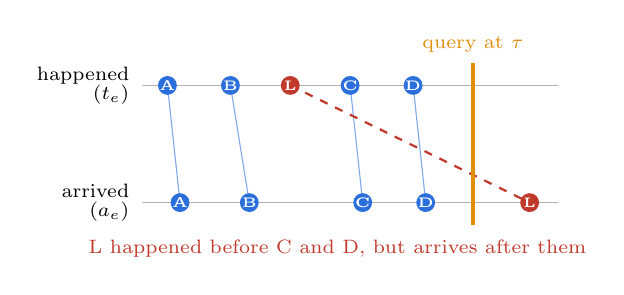
\begin{tikzpicture}[x=0.80cm,y=0.62cm,font=\scriptsize]
 \node[anchor=east,align=right] at (0.25,2.4) {happened\\[-1pt]($t_e$)};
 \node[anchor=east,align=right] at (0.25,0) {arrived\\[-1pt]($a_e$)};
 \draw[gray!60] (0.3,2.4)--(6.9,2.4); \draw[gray!60] (0.3,0)--(6.9,0);
 \foreach \n/\t/\a in {A/0.7/0.9, B/1.7/2.0, C/3.6/3.8, D/4.6/4.8} {
   \draw[cblue!60] (\t,2.4)--(\a,0); \fill[cblue] (\t,2.4) circle (3.4pt) (\a,0) circle (3.4pt);
   \node[white,font=\tiny\bfseries] at (\t,2.4) {\n}; \node[white,font=\tiny\bfseries] at (\a,0) {\n};}
 \draw[cred,thick,dashed] (2.65,2.4)--(6.45,0); \fill[cred] (2.65,2.4) circle (3.4pt) (6.45,0) circle (3.4pt);
 \node[white,font=\tiny\bfseries] at (2.65,2.4) {L}; \node[white,font=\tiny\bfseries] at (6.45,0) {L};
 \draw[corange,very thick] (5.55,-0.45)--(5.55,2.85) node[above,font=\scriptsize]{query at $\tau$};
 \node[text=cred,align=center,font=\scriptsize] at (3.4,-0.95) {L happened before C and D, but arrives after them};
\end{tikzpicture}\\[2pt]{\footnotesize (a) two clocks per event}
\end{minipage}\hfill
\begin{minipage}[b]{0.50\linewidth}\centering
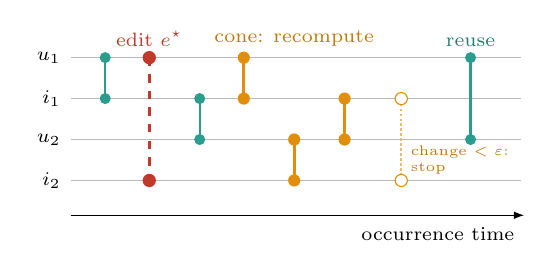
\begin{tikzpicture}[x=0.8cm,y=0.52cm,font=\scriptsize]
 \foreach \y/\l in {3/$u_1$,2/$i_1$,1/$u_2$,0/$i_2$} {\draw[gray!55] (0.25,\y)--(7.4,\y); \node[anchor=east] at (0.25,\y) {\l};}
 \draw[-{Latex[length=1.3mm]}] (0.25,-0.85)--(7.45,-0.85) node[anchor=north east,yshift=-1pt] {occurrence time};
 \foreach \x/\a/\b in {0.8/3/2, 2.3/1/2, 6.6/3/1} {\draw[cgreen,thick] (\x,\a)--(\x,\b); \fill[cgreen] (\x,\a) circle (2pt) (\x,\b) circle (2pt);}
 \draw[cred,very thick,dashed] (1.5,3)--(1.5,0); \fill[cred] (1.5,3) circle (2.4pt) (1.5,0) circle (2.4pt);
 \node[cred,anchor=south,inner sep=1pt] at (1.5,3.2) {edit $e^\star$};
 \foreach \x/\a/\b in {3.0/3/2, 3.8/1/0, 4.6/1/2} {\draw[corange,very thick] (\x,\a)--(\x,\b); \fill[corange] (\x,\a) circle (2.2pt) (\x,\b) circle (2.2pt);}
 \node[corange!85!black,anchor=south,inner sep=1pt] at (3.8,3.2) {cone: recompute};
 \draw[corange!60,thick,densely dotted] (5.5,2)--(5.5,0); \draw[corange,fill=white] (5.5,2) circle (2.2pt); \draw[corange,fill=white] (5.5,0) circle (2.2pt);
 \node[corange!85!black,anchor=west,align=left,inner sep=1pt,font=\tiny] at (5.6,0.5) {change $<\varepsilon$:\\stop};
 \node[cgreen!80!black,anchor=south,inner sep=1pt] at (6.6,3.2) {reuse};
\end{tikzpicture}\\[2pt]{\footnotesize (b) the dependency cone of one edit}
\end{minipage}
\caption{(a) Every event has an occurrence time and an arrival time. At query time $\tau$ the late event L has not
arrived, and when it does, C and D have already been applied without it. (b) Lines are nodes; vertical links are events,
each updating both endpoints. An edit $e^\star$ (late insertion, deletion or amendment) changes every later update that
reads a changed memory (orange). Exact repair recomputes only these, in time order, and copies everything else from a
journal of saved memories (green); $\varepsilon$-repair stops where the change becomes small.}
\label{fig:concept}
\end{figure}


% =========================================================================================================
\section{What changed since the proposal}
\label{sec:changes}

\textbf{Done as planned:} the retroactive memory, the time-ordered neighbour store, edit generators, the SEC graph, and
repair against all baselines, including a StreamTGN-style rebuild \citep{zhang2026streamtgn} and a TIGER-style learned
restart \citep{zhang2023tiger}. \textbf{Changed or added:}
\begin{itemize}
\item \emph{The go/no-go test from the proposal feedback moved our emphasis to deletion.} Full replay is costly and
  buffering is not a cheap fix, but applying late events in arrival order loses almost nothing, so for late events alone
  there is little accuracy to win back. The weight moved to edits that must be honoured exactly, above all deletions,
  where we found the memory leak.
\item \emph{A stronger, calibrated attack.} Besides the model's own score and a probe on the memories, a likelihood-ratio
  attack (LiRA \citep{carlini2022lira}) with counterfactual shadow streams, which we also weaken (partial knowledge of the
  other events, later attacks, fewer candidate pairs) to see how strong an attacker must be.
\item \emph{More models and data:} DyRep (whose update reads the partner's neighbourhood), JODIE, LastFM and tgbl-review
  from TGB \citep{huang2023tgb}; 5 seeds on Wikipedia and Reddit, 3 elsewhere.
\item \emph{A step index} so that repair visits only the steps the cone touches, and an honest account of when it pays
  off (recent edits) and when replay is as fast (old edits on hub-heavy graphs).
\item \emph{A rigorous certificate.} The contraction penalty of the proposal only bounds measured Jacobians; a memory cell
  that contracts by construction makes the error bound hold for every input and enables $\delta$-certified repair.
\item \emph{Deletions of training-period events} (where the weights saw the data too), compared with retraining.
\item \emph{Exact counterfactual explanations:} the effect of deleting any past event on a prediction, compared with
  attention weights.
\item \emph{Not done:} GraphMixer (our memory-free control is a one-layer TGAT-style model) and shadow-model attacks on the
  weights.
\end{itemize}

% =========================================================================================================
\section{Data and processing}
\label{sec:data}

\begin{table}[!htb]
\centering\scriptsize
\caption{Datasets (chronological splits).}
\label{tab:data}
\setlength{\tabcolsep}{4pt}
\begin{tabular}{@{}lrrrrr@{}}
\toprule
 & events & nodes & test events & edge features & days \\
\midrule
Wikipedia & 157,474 & 9,227 & 23,621 & 172 & 31 \\
Reddit & 672,447 & 10,984 & 100,867 & 172 & 31 \\
MOOC & 411,749 & 7,144 & 61,763 & 4 & 30 \\
LastFM & 1,293,103 & 1,980 & 193,966 & 2 & 1,587 \\
tgbl-review & 4,873,540 & 352,637 & 728,919 & 1 & 7,053 \\
SEC Form 4 & 1,048,386 & 69,536 & 156,943 & 25 & 1,003 \\
\bottomrule
\end{tabular}
\end{table}


\textbf{JODIE and TGB.} We load Wikipedia, Reddit, MOOC and LastFM with PyG's \texttt{JODIEDataset} and split by time
70/15/15, as \texttt{TemporalData.train\_val\_test\_split}; tgbl-review comes from the TGB mirror on Hugging Face with TGB's
own split. These datasets have one clock, so test events get arrival times from five delay models with a known ground
truth: \emph{random} (20\% of events late, log-normal delay with a 2-hour median), \emph{active users}, \emph{outage
bursts}, \emph{offline users} and a \emph{slow item shard} (Appendix~\ref{app:details}). The test stream is processed in
steps of 200 events (one day for tgbl-review); an event can be used from the first step after it arrives.

\textbf{SEC Form~4.} We use the point-in-time view of the ZipLime insider-trading data \citep{ziplime2026form4}
(Apache-2.0, built from SEC EDGAR), pinned to one revision. A transaction is an edge from the reporting insider to the
issuer; its occurrence time is the trade date and its arrival time the EDGAR acceptance time; edge features (25-dim)
encode the transaction code, size, price, derivative flag, role and 10b5-1 plan. A Form~4/A row supersedes an earlier row:
at its arrival, the old version is deleted and the new one inserted (\SecAmend{} amendments in the test period). In the test
period \SecLate\% of transactions arrive after the day they happened, the median delay is \SecLagMed{} days, the 99th
percentile \SecLagNinetyNine{} days, and \SecLagFour\% are filed more than 4 days after the trade (the legal deadline is two
business days). To our knowledge no public temporal graph benchmark has real arrival times; we will publish this one.

% =========================================================================================================
\section{Model, repair, attacks and metrics}
\label{sec:model}

\textbf{Model.} PyG's TGN \citep{rossi2020tgn} as in \texttt{examples/tgn.py}: \texttt{TGNMemory} with identity messages and
last-message aggregation, a \texttt{TransformerConv} embedding over each node's last 10 neighbours and an MLP decoder (size
100; batch 200; Adam $10^{-4}$; 15 epochs). When event $e=(u,v,x_e,t_e)$ is processed, endpoint $u$ is updated by
\begin{equation}
s_u \leftarrow F(s_u, s_v, e, \tau_u) = \mathrm{GRU}\big([\,s_u\,\|\,s_v\,\|\,x_e\,\|\,\phi(t_e-\tau_u)\,],\; s_u\big),
\label{eq:tgn}
\end{equation}
where $\tau_u$ is $u$'s previous update time and $\phi$ a learned time encoding; within a step every update reads the memory
from before the step. JODIE uses an RNN memory and a time projection; DyRep's update also attends over the partner's
neighbours, so it reads their memories too.

\textbf{Exact repair.} \texttt{RetroactiveTGNMemory} subclasses \texttt{TGNMemory}, loads the trained weights and keeps a
\emph{journal}: for every update the node, the event, the partner and the memory before and after. After an edit at step
$k_0$ it walks forward and recomputes an update if its event changed or if it reads a memory that differs from the journal
(the cone); every other result is copied. Updates outside the cone see identical inputs, so this returns exactly
$S^\star$, provided the update is batch-invariant: BLAS uses another kernel for single-row products, which in float32
changes the time encoding of multi-day gaps by up to 0.06, so we pad single-row updates (Appendix~\ref{app:fp}). A
\emph{step index} (the steps where each node is updated) lets repair visit only the steps that read a changed memory.
\begin{lstlisting}
mem = RetroactiveTGNMemory.from_trained(tgn.memory, events)   # same weights as the trained TGNMemory
mem.warmup(0, stream.test0)                                    # history, in order
mem.advance(step_events)                                       # one step of the stream (journaled)
mem.edit(insert=late_events, delete=deleted_events)            # change the past (amendment = both)
stats = mem.repair("exact")                                    # or "eps" (eps=0.05), "replay", "khop"
z, last_update = mem(n_id)                                     # as TGNMemory in eval mode
\end{lstlisting}

\textbf{Cheaper repair with a bound.} \emph{$\varepsilon$-repair} keeps the old memory where the recomputed one differs by at
most $\varepsilon\,\|s^{\text{old}}\|$. If every update shrinks memory differences by a factor $\rho<1$, the error stays below
$r/(1-\rho)$, and a per-node bound $b_n\leftarrow\rho\max(b_n,b_o)+\delta_n$ can be tracked online. A trained GRU is not
contractive, so we compare a contraction penalty in training with a cell that contracts by construction,
$s'=(1-a)\odot s+a\odot\tanh(W[s\|p\|x\|\phi]+b)$ with every row of the memory block of $W$ at $\ell_1$ norm at most $c$ and
$a\ge a_{\min}$, so that $\rho=1-a_{\min}(1-c)$ for every input; \emph{$\delta$-certified repair} skips a change only while the
bound stays below $\delta$.

\textbf{Attacks.} We take user--item pairs that first meet in the test period: half (A) are observed and deleted at a request
step, half (B) never happen. The weights were trained before the test period, so anything that separates A from B lives in
the memory. \emph{Query access}: the model's link score, alone and in LiRA with 64 counterfactual shadow streams (random
halves of the candidates observed and then deleted with the method under test; Gaussians with per-pair means). \emph{White-box
access}: a probe on the memories and LiRA on their cosine. AUC 0.5 means the deleted pairs look like pairs that never
happened.

\textbf{Protocol and metrics.} Before step $j$ is scored, every policy turns the events it has received into a memory;
policies share the weights, the negatives and a neighbour store ordered by occurrence time. \emph{Accuracy}: MRR of the true
destination against 100 random and 100 historical negatives. \emph{Cost}: node updates as a multiple of normal in-order
processing, and wall-clock time on a laptop CPU. \emph{Agreement}: top-1 predictions equal to exact repair.
\emph{Privacy}: membership AUC.

% =========================================================================================================
\section{Results so far}
\label{sec:results}

\subsection{Exact repair: exact, and fast for recent edits}
\label{sec:exact}

\begin{table}[t]
\centering\small
\caption{Exact repair on random edits of a 100-step test window (insertions, deletions and amendments; 10\% of the trials edit
2--10 events at once). Max.\ error: largest $|$repaired $-$ reference$|$ over all memory entries, where the reference is a
sequential recomputation of the corrected stream (float32 unless noted). Single edits: share that changes no memory, and
for the others the cone as a share of all updates since the edit (median and 90th percentile; $^\ast$DyRep: median over all
trials). Speed-up: median, over single edits that change a memory, of the time of rollback + replay over the time of exact
repair with the step index (in brackets: walking every step), on an idle laptop CPU; edits that change nothing are
recognised at their own step.}
\label{tab:exact}
\setlength{\tabcolsep}{3.5pt}
\begin{tabular}{@{}lrrrrrrr@{}}
\toprule
 & & & & \multicolumn{3}{c}{single edits} & \\
\cmidrule(lr){5-7}
 & trials & max.\ error & bit-identical & no change & cone & cone p90 & speed-up \\
\midrule
Wikipedia (TGN) & 3,945 & 5.4e-07 & 98\% & 57\% & 0.48\% & 6.8\% & 8.4$\times$ (2.4$\times$) \\
Reddit (TGN) & 2,960 & 9.1e-07 & 72\% & 11\% & 0.38\% & 27.5\% & 5.9$\times$ (2.5$\times$) \\
MOOC (TGN) & 2,960 & 1.0e-06 & 70\% & 54\% & 52.16\% & 80.8\% & 0.9$\times$ (1.2$\times$) \\
LastFM (TGN) & 1,977 & 0 & 100\% & 26\% & 13.74\% & 62.8\% & 1.5$\times$ (1.6$\times$) \\
tgbl-review (TGN) & 982 & 6.0e-08 & 86\% & 6\% & 0.01\% & 0.04\% & 8.2$\times$ (1.8$\times$) \\
Wikipedia (JODIE) & 1,977 & 2.5e-06 & 49\% & 56\% & 0.52\% & 7.8\% & -- \\
Wikipedia (contractive) & 1,977 & 3.0e-08 & 99\% & 56\% & 0.52\% & 7.8\% & -- \\
Wikipedia (DyRep) & 1,500 & 1.6e-05 & -- & 9\%$^\ast$ & 14.75\%$^\ast$ & -- & -- \\
Wikipedia (TGN, float64) & 983 & 0 & 100\% & -- & -- & -- & -- \\
\bottomrule
\end{tabular}
\end{table}


Table~\ref{tab:exact}: over \ExTotalAll{} random insertions, deletions and amendments, the repaired memory equals a fresh
sequential recomputation to within \ExMaxAll{} in float32 and bit for bit in float64; after a deletion the journal, too, is
that of a memory that never saw the events (unit test). \ExNoEffectWiki\% of single edits on Wikipedia change no memory, because
the event is not the latest of its nodes in its step. Among the others the cone is small on Wikipedia and Reddit but large
on hub-heavy graphs (median \ExConeEffMooc\% of the later updates on MOOC), and it grows with the age of the edit. For edits
that change a memory, repair with the step index is \BenchSpeedEffWiki$\times$ faster than replay on Wikipedia,
\BenchSpeedEffReddit$\times$ on Reddit and \BenchSpeedEffReview$\times$ on tgbl-review, but \BenchSpeedEffLastfm$\times$ on
LastFM and \BenchSpeedEffMooc$\times$ on MOOC; on windows of up to 500 steps, edits \AgeOldSteps{} or more steps old are
repaired no faster than they are replayed (Fig.~\ref{fig:age} in the appendix). Repair is the tool for recent edits, replay
for old ones; both are exact. DyRep's cones are far larger (median over all edits \DyrepConeWiki\% of the later updates on
Wikipedia, against \ExConeWiki\% for TGN), because its update reads whole neighbourhoods.

\subsection{Deleting from the log is not enough}
\label{sec:del}

\begin{figure}[t]
\centering
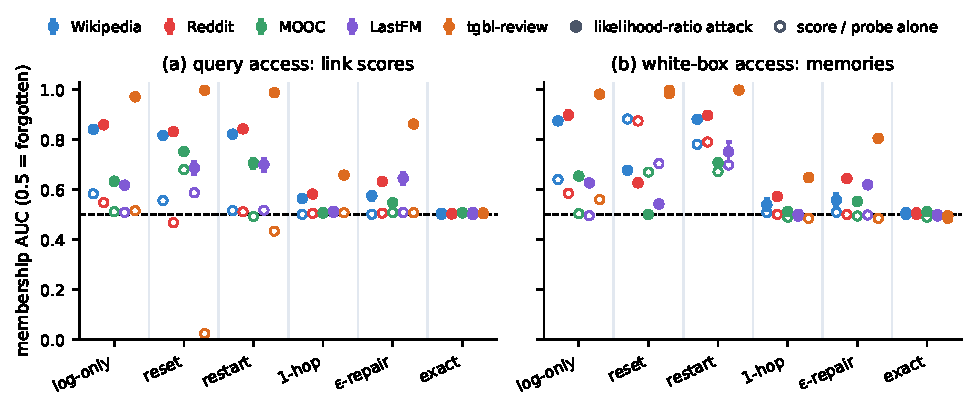
\includegraphics[width=\linewidth]{figures/deletion.pdf}
\caption{Membership AUC after a deletion request (0.5: deleted pairs look like pairs that never happened). (a) Query access:
the model's link score alone (hollow) and in the likelihood-ratio test (filled). (b) White-box access: a probe on the two
memories (hollow) and the likelihood-ratio test on their cosine (filled). Mean $\pm$ std over seeds.}
\label{fig:del}
\end{figure}

With query access alone, log-only deletion is exposed (Fig.~\ref{fig:del}a): the score by itself barely separates A from B
(AUC \RawStoreWiki{} on Wikipedia), but LiRA on the same score reaches \LiraQStoreWiki{} on Wikipedia, \LiraQStoreReddit{} on
Reddit and \LiraQStoreReview{} on tgbl-review, and the memories make it \LiraWStoreWiki, \LiraWStoreReddit{} and
\LiraWStoreReview{} (b). On MOOC the score is at chance even before any deletion, yet LiRA reaches \LiraQStoreMooc. Resetting
the memories and the learned restart fool the score but not LiRA (\LiraQResetWiki{} and \LiraQRestartWiki{} on Wikipedia),
and the probe spots their regenerated memories (\DelProbeResetWiki{} and \DelProbeRestartWiki). The 1-hop rebuild costs about
as much as exact repair and, like $\varepsilon$-repair, leaves a small residue (\LiraQKhopWiki{} and \LiraQEpsWiki). Exact
repair is at chance by construction, at \DelExactCostWiki$\times$ the normal work up to the request on Wikipedia against
\DelReplayCostWiki$\times$ for replay. JODIE and DyRep leak in the same way (LiRA \LiraQStoreJodieWiki{} and
\DyrepLiraQStoreWiki{} on Wikipedia).

\begin{table}[t]
\centering\scriptsize
\caption{The leak under other query-access attackers: LiRA AUC on the link score after log-only deletion (del.) and after
resetting the memories (reset), mean over seeds. The attacker's shadow streams leave out the other test-period events it does
not know; or it attacks 20 or 50 steps after the request; or fewer candidate pairs are unknown at once ($K$; at most 1{,}000
per group by default, 338 on Wikipedia). With partial knowledge and the default $K$, $\varepsilon$-repair, the 1-hop rebuild and
exact repair stay at or below \PartialApproxMax{}; the other rows expose them (Table~\ref{tab:liraknow}). With $K=25$ the AUCs are
noisy: exact repair, which leaks nothing, ranges from \ExactKTwentyFiveMin{} to \ExactKTwentyFiveMax.}
\label{tab:robust}
\setlength{\tabcolsep}{3pt}
\begin{tabular}{@{}lcccccccccc@{}}
\toprule
attacker & \multicolumn{2}{c}{Wikipedia} & \multicolumn{2}{c}{Reddit} & \multicolumn{2}{c}{MOOC} & \multicolumn{2}{c}{LastFM} & \multicolumn{2}{c}{tgbl-review} \\
\cmidrule(lr){2-3} \cmidrule(lr){4-5} \cmidrule(lr){6-7} \cmidrule(lr){8-9} \cmidrule(lr){10-11}
 & del. & reset & del. & reset & del. & reset & del. & reset & del. & reset \\
\midrule
full knowledge, at the request & 0.84 & 0.82 & 0.86 & 0.83 & 0.63 & 0.75 & 0.62 & 0.69 & 0.97 & 1.00 \\
knows 50\% of the other events & 0.70 & 0.74 & 0.65 & 0.77 & 0.53 & 0.73 & 0.51 & 0.66 & 0.57 & 0.97 \\
knows 10\% & 0.65 & 0.67 & 0.61 & 0.73 & 0.50 & 0.72 & 0.51 & 0.64 & 0.53 & 0.97 \\
knows none of them & 0.63 & 0.63 & 0.59 & 0.73 & 0.50 & 0.70 & 0.52 & 0.63 & 0.52 & 0.97 \\
20 steps after the request & 0.84 & 0.81 & 0.87 & 0.85 & 0.65 & 0.72 & 0.65 & 0.67 & 0.97 & 1.00 \\
50 steps after & 0.83 & 0.82 & 0.87 & 0.86 & 0.65 & 0.72 & 0.66 & 0.68 & 0.97 & 1.00 \\
$K=100$ candidate pairs & 0.92 & 0.89 & 0.97 & 0.95 & 0.75 & 0.97 & 0.85 & 0.94 & -- & -- \\
$K=25$ & 0.97 & 0.95 & 0.98 & 0.98 & 0.84 & 1.00 & 0.91 & 0.99 & -- & -- \\
$K=25$, knows 50\% & 0.67 & 0.78 & 0.61 & 0.91 & -- & -- & -- & -- & -- & -- \\
$K=25$, knows none & 0.63 & 0.65 & 0.59 & 0.80 & -- & -- & -- & -- & -- & -- \\
\bottomrule
\end{tabular}
\end{table}


\textbf{How strong must the attacker be?} Table~\ref{tab:robust}: an attacker who knows none of the other test-period events
still detects log-only deletion on Wikipedia and Reddit (\LiraKnowNoneQStoreWiki{} and \LiraKnowNoneQStoreReddit) and resets
everywhere (\LiraKnowNoneQResetWiki--\LiraKnowNoneQResetReview); 50 steps after the request the leak is unchanged
(\LiraAfterFiftyQStoreWiki{} on Wikipedia); with fewer candidate pairs unknown at once ($K=25$) log-only deletion is exposed
with AUC \LiraKTwentyFiveQStoreWiki{} on Wikipedia and \LiraKTwentyFiveQStoreMooc{} on MOOC. The residues of
$\varepsilon$-repair and the 1-hop rebuild are visible only to an attacker who knows almost every other event.

\textbf{Training-period deletions.} When the weights saw the events too, we compare with retraining from scratch without them
(Table~\ref{tab:traindel} in the appendix). \TrainDelText

\subsection{Cheaper repair with a guarantee}
\label{sec:cert}

Standard TGNs are not contractive (local Jacobian norms sum to \ConVanillaJsum, median), so our bound does not apply to them.
A contraction penalty makes \CertEightFive\% of the updates contract at $\rho=0.85$ for \MrrLossEightFive{} MRR points, but only
at the states it measured. The contractive cell contracts for every input: its proven per-node bound held in all trials and
was within \RigRatioNineCell$\times$ of the true worst error (median), and $\delta$-certified repair with $\delta=0.02$
recomputes \CertRepairCostNineCell$\times$ the updates of exact repair while keeping every memory within 0.02 of the exact one;
the price is \MrrLossNineCell{} MRR points at $\rho\le0.9$ on Wikipedia (Table~\ref{tab:cert} in the appendix).

\subsection{Late events and SEC Form~4}
\label{sec:late}

Applying late events on arrival, out of order, changes MRR by \ArrivalRelWiki\%, \ArrivalRelReddit\% and \ArrivalRelMooc\% on
Wikipedia, Reddit and MOOC relative to exact repair, within the spread over seeds; a one-hour buffer changes it by
\BufOneRelWiki\%, \BufOneRelReddit\% and \BufOneRelMooc\%, because it holds back every recent event, not only the late ones
(all delay models: Table~\ref{tab:delays}; all policies: Table~\ref{tab:late}, both in the appendix). On SEC Form~4, with
real delays and amendments, every policy is within \SecSpreadPct\% of exact repair except dropping late events
(\SecDropRel\%), while seeing every event on time would gain \SecOracleRel\%: what lateness costs is the information that
has not arrived, which no repair recovers. Exact repair is not free in wall-clock time (\BenchStreamExactMsWiki{} ms per step
of 200 Wikipedia events against \BenchStreamArrivalMsWiki{} ms in arrival order and \BenchStreamReplayMsWiki{} ms for replay),
so for late events repair is a matter of correctness, not of accuracy.

\subsection{Exact counterfactual explanations}
\label{sec:infl}

Deleting each of a user's last 20 events in turn and repairing gives the exact effect of every event on a prediction (up to
200 predictions per model, 3 seeds; Fig.~\ref{fig:infl} in the appendix). About half of the influence (\MemChannelWiki\% on
Wikipedia) flows through the memory, and \ShareOutsideWiki\% comes from events outside the 10 the attention layer sees. The
most-attended event is the most influential one for the neighbour-list channel in \AttTopOneListWiki\% of the predictions
on Wikipedia (chance 10\%), but for the total effect only in \AttTopOneTotalWiki\% (\AttTopOneTotalMooc\% on MOOC):
attention only partly explains what it weighs, and not the prediction.

% =========================================================================================================
\section{Next steps (until December 10)}
\label{sec:next}

\begin{itemize}
\item \textbf{Nov 11--24} (Lexi): the Medium blog post (motivation, the cone animation, PyG snippets, the deletion attack,
  results), reviewed by the course staff before publishing; the Colab notebook as its companion (already runs end to end
  with saved outputs).
\item \textbf{Nov 11--24} (Yijin): a shadow-model attack on the weights for training-period deletions; GraphMixer or
  DyGFormer as a stronger memory-free baseline; release of the SEC two-clock graph.
\item \textbf{Nov 25--Dec 10} (both): figures and text polish, the public GitHub repository with every job list, and an
  optional GPU version of the repair loop.
\end{itemize}

\section{Questions we would like feedback on}
\label{sec:feedback}

\begin{enumerate}
\item Is the privacy finding (log-only deletion leaks through the memory; resets leave a fingerprint) the right main story for
  the blog post, with exact repair as the fix and late events as a secondary result?
\item Our strongest attacker knows the weights and the other events; weaker ones still find log-only deletion on Wikipedia
  and Reddit. Which attacker would you consider realistic enough to put first?
\item Exact repair beats replay only for recent edits. Is it acceptable to recommend replay for old edits (both are exact),
  or should we invest in a faster (GPU) repair before the final?
\item On SEC most insiders trade a single stock, so link prediction is easy (MRR of exact repair \SecExactMrr). Would a
  node-level task be a better showcase for the real two-clock data?
\end{enumerate}

\paragraph{Code.} \url{\CodeURL}: the \texttt{lategraph} package, 18 unit tests (our kernel equals PyG's \texttt{TGNMemory};
exact repair equals recomputation in float32 and float64; the step index equals the full walk bit for bit; the journal is
purged), all experiment scripts with the job lists behind every number in this report, the JSON results, and a Colab notebook
with saved outputs that trains a TGN, repairs a late event, runs the streaming evaluation, the deletion attack and the
contractive cell, and redraws every result in about 20 minutes on a CPU.

\bibliographystyle{abbrvnat}
\small
\bibliography{references}
\normalsize

\newpage
\appendix

\section{Training and evaluation details}
\label{app:details}

\textbf{Delay models.} \emph{Random}: 20\% of the test events are late, with a log-normal delay of median 2 hours ($\sigma=1$;
tgbl-review: median 2 days); \emph{active}: the 5\% most active users send half of their events late; \emph{burst}: 4 outages
of 3 hours, during each of which the events of a random half of the users are held; \emph{offline}: 20\% of the users upload
their events every 6 hours; \emph{item shard}: 20\% of the items live on a slow shard and half of their events are late.

\textbf{Attacks.} Deletion pairs: user--item pairs whose first interaction lies in the first half of the test period and whose
user has at least three other events, at most 1{,}000 per group (\LiraPairsWiki{} on Wikipedia); the request is at the
middle of the test period. LiRA: 64 shadow streams (16 for DyRep and tgbl-review). Weaker attackers: with knowledge $f$, a
fixed random $1-f$ of the other test-period events is left out of every shadow stream; with a delay of $k$ steps, target and
shadows process $k$ more steps before the attack; with $K<1{,}000$, fewer candidate pairs are drawn. The probe is a logistic
regression on memory features trained with 5-fold cross-validation on the target's own labels.

\textbf{Models.} Memory, time and embedding size 100, 10 neighbours, 2-head \texttt{TransformerConv}, batch 200, Adam
$10^{-4}$, one random negative per positive, best epoch by validation AP (15 epochs; SEC 10; tgbl-review 6). The contraction
penalty uses 64 sampled updates per batch and $\lambda=10$; the contractive cell uses $c=0.5$ and $a_{\min}=(1-\rho)/(1-c)$.

\section{Why float32 broke our first exactness test}
\label{app:fp}

The time encoding is $\phi(\Delta t)=\cos(\omega\Delta t+b)$ with trained $|\omega|$ up to about 1 and $\Delta t$ in seconds,
so $\omega\Delta t$ reaches $10^6$ for a gap of about 12 days, where adjacent float32 numbers are $0.0625$ apart.
\texttt{torch.nn.Linear} uses a matrix--vector kernel when the batch has one row and a matrix--matrix kernel otherwise; the two
round $\omega\Delta t+b$ differently, and the cosine turns a one-ulp difference into up to $0.06$. Exact repair recomputes
small subsets of a step while the reference recomputes whole steps, so without padding \ExNoPadFail\% of the trials disagreed
by more than $10^{-5}$. Padding single-row updates to two rows removes these errors; the remaining differences come from the
summation order of batched kernels, and in float64 every repaired memory was bit-identical to the reference.

\section{More results}
\label{app:extra}

\begin{figure}[!htb]
\centering
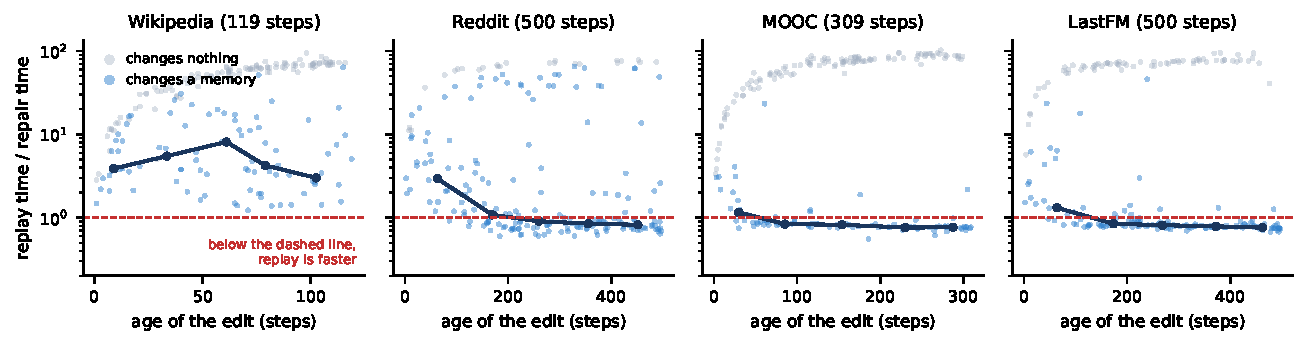
\includegraphics[width=\linewidth]{figures/repair_age.pdf}
\caption{Time of rollback + replay over the time of exact repair (step index) for single edits at random positions of the
longest available test window, against the age of the edit; line: median over edits that change a memory.}
\label{fig:age}
\end{figure}

\begin{table}[t]
\centering\scriptsize
\caption{Deleting training-period pairs (membership AUC of the link score / the memory probe at the deployment start; mean
$\pm$ std over seeds, number of seeds in brackets). ``Recent'': pairs from the last 20\% of the training period. Last row:
time of one exact memory repair for a single pair / of recomputing the memory over the whole history with fixed weights
(one batched pass, idle machine) / of retraining one model.}
\label{tab:traindel}
\setlength{\tabcolsep}{3pt}
\begin{tabular}{@{}lcccccccc@{}}
\toprule
 & \multicolumn{2}{c}{Wikipedia (5)} & \multicolumn{2}{c}{Reddit (3)} & \multicolumn{2}{c}{MOOC (3)} & \multicolumn{2}{c}{Wikipedia, recent (3)} \\
 & score & probe & score & probe & score & probe & score & probe \\
\midrule
no deletion & 0.55\,{\scriptsize$\pm$0.02} & 0.52\,{\scriptsize$\pm$0.01} & 0.52\,{\scriptsize$\pm$0.01} & 0.51\,{\scriptsize$\pm$0.01} & 0.49\,{\scriptsize$\pm$0.03} & 0.52\,{\scriptsize$\pm$0.01} & 0.58\,{\scriptsize$\pm$0.02} & 0.54\,{\scriptsize$\pm$0.02} \\
log-only & 0.52\,{\scriptsize$\pm$0.02} & 0.52\,{\scriptsize$\pm$0.02} & 0.51\,{\scriptsize$\pm$0.01} & 0.51\,{\scriptsize$\pm$0.01} & 0.49\,{\scriptsize$\pm$0.03} & 0.52\,{\scriptsize$\pm$0.02} & 0.54\,{\scriptsize$\pm$0.01} & 0.54\,{\scriptsize$\pm$0.02} \\
memory repair & 0.50\,{\scriptsize$\pm$0.02} & 0.51\,{\scriptsize$\pm$0.01} & 0.50\,{\scriptsize$\pm$0.01} & 0.50\,{\scriptsize$\pm$0.01} & 0.49\,{\scriptsize$\pm$0.03} & 0.52\,{\scriptsize$\pm$0.02} & 0.50\,{\scriptsize$\pm$0.01} & 0.50\,{\scriptsize$\pm$0.03} \\
memory repair + fine-tune & 0.49\,{\scriptsize$\pm$0.00} & 0.50\,{\scriptsize$\pm$0.03} & 0.49\,{\scriptsize$\pm$0.01} & 0.51\,{\scriptsize$\pm$0.05} & 0.49\,{\scriptsize$\pm$0.03} & 0.48\,{\scriptsize$\pm$0.02} & 0.51\,{\scriptsize$\pm$0.02} & 0.48\,{\scriptsize$\pm$0.03} \\
retrain (reference) & 0.52\,{\scriptsize$\pm$0.02} & 0.51\,{\scriptsize$\pm$0.02} & 0.50\,{\scriptsize$\pm$0.02} & 0.50\,{\scriptsize$\pm$0.01} & 0.49\,{\scriptsize$\pm$0.02} & 0.50\,{\scriptsize$\pm$0.03} & 0.49\,{\scriptsize$\pm$0.02} & 0.47\,{\scriptsize$\pm$0.02} \\
\midrule
cost: repair / recompute / retrain & \multicolumn{2}{c}{0.48 s / 0.28 s / 5 min} & \multicolumn{2}{c}{5.58 s / 1.60 s / 32 min} & \multicolumn{2}{c}{0.82 s / 0.53 s / 7 min} & \multicolumn{2}{c}{0.08 s / 0.28 s / 4 min} \\
\bottomrule
\end{tabular}
\end{table}

\begin{table}[t]
\centering\scriptsize
\caption{Contraction and the error bound on Wikipedia ($\varepsilon=0.05$; 100 random deletions per model and seed). Certified:
updates with $\|J_{\text{own}}\|+\|J_{\text{partner}}\|<1$ (all updates for the contractive cell, which contracts by
construction). Bound held: share of trials in which the per-node bound held for every node (first order for the
GRU, proven for the cell). $\delta$-cert.: updates recomputed by $\delta$-certified repair ($\delta=0.02$) relative to exact repair.}
\label{tab:cert}
\setlength{\tabcolsep}{3pt}
\begin{tabular}{@{}lrrrrrr@{}}
\toprule
 & val.\ AP & test MRR & certified (\%) & bound held (\%) & bound / error & $\delta$-cert.\ cost \\
\midrule
standard TGN (GRU) & 0.965\,{\scriptsize$\pm$0.002} & 0.643\,{\scriptsize$\pm$0.018} & 0.0\,{\scriptsize$\pm$0.0} & 100 & 26.7 & -- \\
penalty, $\rho=0.95$ & 0.956\,{\scriptsize$\pm$0.001} & 0.656\,{\scriptsize$\pm$0.005} & 20.3\,{\scriptsize$\pm$1.6} & 100 & 1.2 & -- \\
penalty, $\rho=0.85$ & 0.951\,{\scriptsize$\pm$0.000} & 0.630\,{\scriptsize$\pm$0.007} & 99.2\,{\scriptsize$\pm$0.1} & 100 & 1.1 & -- \\
penalty, $\rho=0.75$ & 0.946\,{\scriptsize$\pm$0.001} & 0.619\,{\scriptsize$\pm$0.006} & 99.9\,{\scriptsize$\pm$0.0} & 100 & 1.0 & -- \\
penalty, $\rho=0.85$, $\lambda=1$ & 0.952\,{\scriptsize$\pm$0.001} & 0.630\,{\scriptsize$\pm$0.007} & 81.7\,{\scriptsize$\pm$3.3} & 100 & 1.1 & -- \\
penalty, $\rho=0.85$, $\lambda=100$ & 0.948\,{\scriptsize$\pm$0.000} & 0.621\,{\scriptsize$\pm$0.002} & 99.8\,{\scriptsize$\pm$0.0} & 100 & 1.1 & -- \\
contractive cell, $\rho\le0.95$ & 0.939\,{\scriptsize$\pm$0.001} & 0.582\,{\scriptsize$\pm$0.010} & 100 & 100 (proven) & 5.1 & 0.46 \\
contractive cell, $\rho\le0.9$ & 0.939\,{\scriptsize$\pm$0.002} & 0.580\,{\scriptsize$\pm$0.016} & 100 & 100 (proven) & 5.2 & 0.45 \\
contractive cell, $\rho\le0.8$ & 0.939\,{\scriptsize$\pm$0.002} & 0.583\,{\scriptsize$\pm$0.012} & 100 & 100 (proven) & 5.2 & 0.44 \\
contractive cell, $\rho\le0.95$, $c=0.7$ & 0.942\,{\scriptsize$\pm$0.002} & 0.587\,{\scriptsize$\pm$0.016} & 100 & 100 (proven) & 5.6 & 0.47 \\
contractive cell, $\rho\le0.99$, $c=0.9$ & 0.946\,{\scriptsize$\pm$0.001} & 0.606\,{\scriptsize$\pm$0.008} & 100 & 100 (proven) & 7.0 & 0.50 \\
\bottomrule
\end{tabular}
\end{table}

\begin{table}[t]
\centering\scriptsize
\caption{Late events (random delays), steps of 200 events, mean $\pm$ std over seeds. MRR changes are relative to exact repair
and paired within each seed; compute is in multiples of normal in-order processing. $^\ddagger$Daily steps (the timestamps
are days), delays with a median of 2 days, the first 200 test days with 300 queries per day; buffers of 1 and 4 days.
$^\S$Real arrival times and amendments, daily steps; buffers of 1 and 4 days.}
\label{tab:late}
\setlength{\tabcolsep}{3pt}
\begin{tabular}{@{}lcccccc@{}}
\toprule
 & Wikipedia & Reddit & MOOC & LastFM & tgbl-review$^\ddagger$ & SEC$^\S$ \\
\midrule
seeds & 5 & 5 & 5 & 3 & 3 & 5 \\
test events that arrive late (\%) & 18.0 & 20.0 & 19.8 & 11.8 & 15.1 & 93.0 \\
MRR of exact repair & 0.640\,{\scriptsize$\pm$0.018} & 0.739\,{\scriptsize$\pm$0.019} & 0.152\,{\scriptsize$\pm$0.082} & 0.083\,{\scriptsize$\pm$0.021} & 0.359\,{\scriptsize$\pm$0.033} & 0.653\,{\scriptsize$\pm$0.022} \\
\midrule
MRR vs.\ exact repair (\%) &  &  &  &  &  &  \\
\quad oracle (all on time) & +0.45\,{\scriptsize$\pm$0.16} & +0.13\,{\scriptsize$\pm$0.08} & +0.43\,{\scriptsize$\pm$1.35} & -0.23\,{\scriptsize$\pm$0.41} & +0.04\,{\scriptsize$\pm$0.04} & +1.74\,{\scriptsize$\pm$0.09} \\
\quad arrival order & +0.13\,{\scriptsize$\pm$0.56} & -0.13\,{\scriptsize$\pm$0.10} & +0.13\,{\scriptsize$\pm$2.84} & +2.32\,{\scriptsize$\pm$2.81} & +1.37\,{\scriptsize$\pm$4.73} & +0.07\,{\scriptsize$\pm$0.17} \\
\quad drop late events & +0.04\,{\scriptsize$\pm$0.56} & -0.06\,{\scriptsize$\pm$0.06} & +0.40\,{\scriptsize$\pm$0.34} & +1.77\,{\scriptsize$\pm$2.22} & +0.12\,{\scriptsize$\pm$0.24} & -0.91\,{\scriptsize$\pm$0.30} \\
\quad buffer 1 h (1 day$^{\ddagger\S}$) & -4.92\,{\scriptsize$\pm$0.86} & -1.53\,{\scriptsize$\pm$0.83} & -11.33\,{\scriptsize$\pm$9.19} & -4.74\,{\scriptsize$\pm$8.69} & +2.08\,{\scriptsize$\pm$5.00} & -0.06\,{\scriptsize$\pm$0.09} \\
\quad buffer 4 h (4 days) & -9.49\,{\scriptsize$\pm$0.71} & -1.99\,{\scriptsize$\pm$0.52} & -14.24\,{\scriptsize$\pm$10.94} & -2.72\,{\scriptsize$\pm$5.79} & +0.24\,{\scriptsize$\pm$2.23} & -0.24\,{\scriptsize$\pm$0.09} \\
\quad $\varepsilon$-repair, $\varepsilon=0.05$ & +0.01\,{\scriptsize$\pm$0.05} & -0.01\,{\scriptsize$\pm$0.03} & +0.32\,{\scriptsize$\pm$0.24} & +0.09\,{\scriptsize$\pm$0.21} & +0.01\,{\scriptsize$\pm$0.05} & -0.00\,{\scriptsize$\pm$0.01} \\
\midrule
compute ($\times$ normal processing) &  &  &  &  &  &  \\
\quad full replay & 16.72 & 69.37 & 48.97 & 5.88 & 34.48 & 54.86 \\
\quad exact repair (cone) & 1.30 & 13.69 & 23.10 & 1.11 & 1.10 & 1.06 \\
\quad 1-hop rebuild & 1.27 & 7.18 & 21.92 & 1.10 & -- & 1.05 \\
\quad $\varepsilon$-repair & 1.24 & 1.89 & 2.20 & 1.08 & 1.07 & 1.04 \\
\midrule
top-1 prediction as exact repair (\%) &  &  &  &  &  &  \\
\quad arrival order & 78.7 & 91.6 & 69.7 & 79.6 & 82.0 & 84.9 \\
\quad $\varepsilon$-repair & 99.3 & 98.4 & 90.7 & 98.3 & 99.4 & 99.8 \\
\quad 1-hop rebuild & 99.7 & 99.8 & 100.0 & 100.0 & -- & 99.9 \\
\bottomrule
\end{tabular}
\end{table}

\begin{table}[!htb]
\centering\scriptsize
\caption{Every delay setting: MRR change relative to exact repair (\%) and compute (multiples of normal processing), mean
over seeds.}
\label{tab:delays}
\setlength{\tabcolsep}{2.4pt}
\resizebox{\linewidth}{!}{%
\begin{tabular}{@{}lllrrrrrrrrrrr@{}}
\toprule
 & delay model & step & seeds & late \% & arrival & drop & buffer 1h & buffer 4h & $\varepsilon$=0.05 & replay & exact & $\varepsilon$=0.05 & 1-hop \\
\midrule
Wikipedia & random & 200 & 5 & 18.0 & +0.13 & +0.04 & -4.92 & -9.49 & +0.01 & 16.72 & 1.30 & 1.24 & 1.27 \\
Wikipedia & random & 50 & 5 & 19.9 & -0.17 & -0.14 & -7.92 & -13.29 & +0.02 & 37.22 & 1.73 & 1.46 & 1.58 \\
Wikipedia & active users & 200 & 5 & 18.9 & +0.13 & -0.01 & -4.45 & -9.29 & +0.02 & 16.68 & 1.30 & 1.25 & 1.27 \\
Wikipedia & outages & 200 & 5 & 3.5 & -0.02 & -0.05 & -5.05 & -9.61 & -0.00 & 1.07 & 1.01 & 1.01 & 1.01 \\
Wikipedia & offline users & 200 & 3 & 16.7 & -0.07 & -1.91 & -3.94 & -8.00 & +0.01 & 5.79 & 1.07 & 1.06 & 1.06 \\
Wikipedia & slow item shard & 200 & 3 & 8.8 & +0.05 & -0.22 & -5.16 & -9.62 & -0.02 & 13.56 & 1.14 & 1.11 & 1.12 \\
Reddit & random & 200 & 5 & 20.0 & -0.13 & -0.06 & -1.53 & -1.99 & -0.01 & 69.37 & 13.69 & 1.89 & 7.18 \\
Reddit & active users & 200 & 5 & 12.4 & -0.07 & +0.01 & -1.54 & -1.96 & +0.00 & 59.84 & 12.69 & 1.64 & 6.16 \\
Reddit & outages & 200 & 5 & 5.3 & -0.01 & -0.03 & -1.17 & -1.81 & +0.00 & 1.13 & 1.04 & 1.04 & 1.04 \\
Reddit & offline users & 200 & 3 & 19.1 & -0.08 & -0.35 & -1.47 & -1.80 & -0.02 & 24.07 & 2.94 & 1.62 & 2.21 \\
Reddit & slow item shard & 200 & 3 & 13.7 & -0.05 & -0.15 & -1.36 & -1.98 & +0.01 & 60.15 & 9.15 & 1.54 & 3.25 \\
MOOC & random & 200 & 5 & 19.8 & +0.13 & +0.40 & -11.33 & -14.24 & +0.32 & 48.97 & 23.10 & 2.20 & 21.92 \\
MOOC & random & 50 & 5 & 20.0 & -2.31 & +0.24 & -12.78 & -16.59 & +0.37 & 118.37 & 77.80 & 2.41 & 58.65 \\
MOOC & active users & 200 & 5 & 4.3 & +0.25 & +0.28 & -9.40 & -13.13 & +0.03 & 30.55 & 9.79 & 1.28 & 6.63 \\
MOOC & outages & 200 & 5 & 5.6 & +0.20 & +0.10 & -9.57 & -13.31 & +0.03 & 1.14 & 1.09 & 1.07 & 1.09 \\
MOOC & offline users & 200 & 3 & 18.6 & -0.04 & +0.08 & -10.46 & -13.29 & +0.51 & 17.48 & 7.89 & 1.68 & 4.38 \\
MOOC & slow item shard & 200 & 3 & 10.4 & -0.90 & -0.01 & -11.87 & -14.17 & +0.09 & 39.53 & 15.70 & 1.63 & 12.70 \\
LastFM & random & 200 & 3 & 11.8 & +2.32 & +1.77 & -4.74 & -2.72 & +0.09 & 5.88 & 1.11 & 1.08 & 1.10 \\
LastFM & active users & 200 & 3 & 6.0 & -0.07 & +0.73 & -0.12 & -3.31 & +0.02 & 4.89 & 1.06 & 1.05 & 1.06 \\
LastFM & outages & 200 & 3 & 0.0 & +0.02 & +0.01 & -0.23 & -3.10 & -0.00 & 1.00 & 1.00 & 1.00 & 1.00 \\
\bottomrule
\end{tabular}}
\end{table}

\begin{table}[!htb]
\centering\scriptsize
\caption{The likelihood-ratio attack for every attacker variant and deletion method: AUC with query access (LiRA on the link
score) / with white-box access (LiRA on the cosine of the two memories), mean over seeds (5 for Wikipedia and Reddit, 3
otherwise; 16 shadow streams for tgbl-review, 64 otherwise).}
\label{tab:liraknow}
\setlength{\tabcolsep}{3pt}
\begin{tabular}{@{}llcccccc@{}}
\toprule
 & attacker & log-only & reset & restart & 1-hop & $\varepsilon$-repair & exact \\
\midrule
Wikipedia & full knowledge, at the request & 0.84\,/\,0.87 & 0.82\,/\,0.68 & 0.82\,/\,0.88 & 0.56\,/\,0.54 & 0.58\,/\,0.56 & 0.50\,/\,0.50 \\
 & knows 50\% of the other events & 0.70\,/\,0.80 & 0.74\,/\,0.68 & 0.63\,/\,0.77 & 0.50\,/\,0.49 & 0.50\,/\,0.49 & 0.50\,/\,0.50 \\
 & knows 10\% & 0.65\,/\,0.75 & 0.67\,/\,0.68 & 0.58\,/\,0.70 & 0.51\,/\,0.50 & 0.51\,/\,0.50 & 0.50\,/\,0.50 \\
 & knows none of them & 0.63\,/\,0.73 & 0.63\,/\,0.68 & 0.57\,/\,0.68 & 0.50\,/\,0.50 & 0.50\,/\,0.50 & 0.50\,/\,0.50 \\
 & 20 steps after the request & 0.84\,/\,0.87 & 0.81\,/\,0.85 & 0.81\,/\,0.85 & 0.55\,/\,0.54 & 0.54\,/\,0.56 & 0.50\,/\,0.50 \\
 & 50 steps after & 0.83\,/\,0.86 & 0.82\,/\,0.84 & 0.81\,/\,0.84 & 0.56\,/\,0.53 & 0.53\,/\,0.55 & 0.50\,/\,0.49 \\
 & $K=100$ candidate pairs & 0.92\,/\,0.95 & 0.89\,/\,0.85 & 0.92\,/\,0.96 & 0.63\,/\,0.60 & 0.64\,/\,0.59 & 0.50\,/\,0.50 \\
 & $K=25$ & 0.97\,/\,0.98 & 0.95\,/\,0.95 & 0.98\,/\,1.00 & 0.70\,/\,0.69 & 0.73\,/\,0.74 & 0.50\,/\,0.51 \\
 & $K=25$, knows 50\% & 0.67\,/\,0.80 & 0.78\,/\,0.96 & 0.63\,/\,0.84 & 0.47\,/\,0.60 & 0.49\,/\,0.49 & 0.50\,/\,0.50 \\
 & $K=25$, knows none & 0.63\,/\,0.72 & 0.65\,/\,0.95 & 0.51\,/\,0.68 & 0.50\,/\,0.50 & 0.50\,/\,0.50 & 0.50\,/\,0.50 \\
\midrule
Reddit & full knowledge, at the request & 0.86\,/\,0.90 & 0.83\,/\,0.63 & 0.84\,/\,0.90 & 0.58\,/\,0.57 & 0.63\,/\,0.64 & 0.50\,/\,0.51 \\
 & knows 50\% of the other events & 0.65\,/\,0.73 & 0.77\,/\,0.63 & 0.56\,/\,0.68 & 0.51\,/\,0.51 & 0.52\,/\,0.50 & 0.51\,/\,0.50 \\
 & knows 10\% & 0.61\,/\,0.67 & 0.73\,/\,0.63 & 0.52\,/\,0.62 & 0.50\,/\,0.51 & 0.50\,/\,0.50 & 0.51\,/\,0.50 \\
 & knows none of them & 0.59\,/\,0.65 & 0.73\,/\,0.63 & 0.53\,/\,0.62 & 0.50\,/\,0.50 & 0.50\,/\,0.50 & 0.50\,/\,0.50 \\
 & 20 steps after the request & 0.87\,/\,0.90 & 0.85\,/\,0.87 & 0.84\,/\,0.88 & 0.57\,/\,0.56 & 0.63\,/\,0.65 & 0.51\,/\,0.49 \\
 & 50 steps after & 0.87\,/\,0.90 & 0.86\,/\,0.87 & 0.85\,/\,0.87 & 0.56\,/\,0.57 & 0.63\,/\,0.65 & 0.51\,/\,0.50 \\
 & $K=100$ candidate pairs & 0.97\,/\,0.98 & 0.95\,/\,0.93 & 0.98\,/\,0.99 & 0.71\,/\,0.74 & 0.83\,/\,0.82 & 0.46\,/\,0.49 \\
 & $K=25$ & 0.98\,/\,0.98 & 0.98\,/\,0.98 & 0.99\,/\,1.00 & 0.76\,/\,0.78 & 0.94\,/\,0.87 & 0.46\,/\,0.44 \\
 & $K=25$, knows 50\% & 0.61\,/\,0.75 & 0.91\,/\,0.97 & 0.55\,/\,0.71 & 0.50\,/\,0.55 & 0.49\,/\,0.49 & 0.51\,/\,0.60 \\
 & $K=25$, knows none & 0.59\,/\,0.73 & 0.80\,/\,0.97 & 0.47\,/\,0.63 & 0.50\,/\,0.50 & 0.50\,/\,0.50 & 0.50\,/\,0.50 \\
\midrule
MOOC & full knowledge, at the request & 0.63\,/\,0.65 & 0.75\,/\,0.50 & 0.71\,/\,0.71 & 0.51\,/\,0.51 & 0.55\,/\,0.55 & 0.51\,/\,0.51 \\
 & knows 50\% of the other events & 0.53\,/\,0.55 & 0.73\,/\,0.50 & 0.54\,/\,0.56 & 0.49\,/\,0.50 & 0.49\,/\,0.51 & 0.49\,/\,0.50 \\
 & knows 10\% & 0.50\,/\,0.51 & 0.72\,/\,0.50 & 0.53\,/\,0.52 & 0.50\,/\,0.49 & 0.49\,/\,0.48 & 0.50\,/\,0.49 \\
 & knows none of them & 0.50\,/\,0.50 & 0.70\,/\,0.50 & 0.51\,/\,0.51 & 0.50\,/\,0.50 & 0.50\,/\,0.50 & 0.50\,/\,0.50 \\
 & 20 steps after the request & 0.65\,/\,0.66 & 0.72\,/\,0.74 & 0.69\,/\,0.71 & 0.50\,/\,0.50 & 0.54\,/\,0.55 & 0.50\,/\,0.50 \\
 & 50 steps after & 0.65\,/\,0.66 & 0.72\,/\,0.73 & 0.69\,/\,0.71 & 0.51\,/\,0.50 & 0.54\,/\,0.55 & 0.51\,/\,0.50 \\
 & $K=100$ candidate pairs & 0.75\,/\,0.78 & 0.97\,/\,0.68 & 0.94\,/\,0.96 & 0.52\,/\,0.49 & 0.66\,/\,0.68 & 0.52\,/\,0.53 \\
 & $K=25$ & 0.84\,/\,0.85 & 1.00\,/\,0.90 & 0.98\,/\,0.99 & 0.63\,/\,0.60 & 0.76\,/\,0.71 & 0.46\,/\,0.52 \\
\midrule
LastFM & full knowledge, at the request & 0.62\,/\,0.63 & 0.69\,/\,0.54 & 0.70\,/\,0.75 & 0.51\,/\,0.50 & 0.65\,/\,0.62 & 0.50\,/\,0.50 \\
 & knows 50\% of the other events & 0.51\,/\,0.51 & 0.66\,/\,0.54 & 0.53\,/\,0.66 & 0.50\,/\,0.50 & 0.51\,/\,0.50 & 0.50\,/\,0.50 \\
 & knows 10\% & 0.51\,/\,0.51 & 0.64\,/\,0.54 & 0.53\,/\,0.62 & 0.50\,/\,0.49 & 0.50\,/\,0.51 & 0.50\,/\,0.50 \\
 & knows none of them & 0.52\,/\,0.50 & 0.63\,/\,0.54 & 0.52\,/\,0.58 & 0.50\,/\,0.50 & 0.50\,/\,0.50 & 0.50\,/\,0.50 \\
 & 20 steps after the request & 0.65\,/\,0.64 & 0.67\,/\,0.63 & 0.67\,/\,0.67 & 0.50\,/\,0.50 & 0.65\,/\,0.62 & 0.50\,/\,0.50 \\
 & 50 steps after & 0.66\,/\,0.63 & 0.68\,/\,0.66 & 0.66\,/\,0.64 & 0.51\,/\,0.51 & 0.65\,/\,0.63 & 0.50\,/\,0.50 \\
 & $K=100$ candidate pairs & 0.85\,/\,0.83 & 0.94\,/\,0.87 & 0.94\,/\,0.99 & 0.54\,/\,0.51 & 0.86\,/\,0.82 & 0.50\,/\,0.50 \\
 & $K=25$ & 0.91\,/\,0.93 & 0.99\,/\,0.97 & 0.98\,/\,0.99 & 0.72\,/\,0.60 & 0.91\,/\,0.92 & 0.54\,/\,0.53 \\
\midrule
tgbl-review & full knowledge, at the request & 0.97\,/\,0.98 & 1.00\,/\,0.98 & 0.99\,/\,1.00 & 0.66\,/\,0.65 & 0.86\,/\,0.81 & 0.50\,/\,0.50 \\
 & knows 50\% of the other events & 0.57\,/\,0.62 & 0.97\,/\,0.98 & 0.62\,/\,0.73 & 0.49\,/\,0.50 & 0.51\,/\,0.49 & 0.50\,/\,0.50 \\
 & knows 10\% & 0.53\,/\,0.54 & 0.97\,/\,0.98 & 0.55\,/\,0.62 & 0.50\,/\,0.50 & 0.49\,/\,0.50 & 0.50\,/\,0.50 \\
 & knows none of them & 0.52\,/\,0.52 & 0.97\,/\,0.98 & 0.53\,/\,0.62 & 0.50\,/\,0.50 & 0.50\,/\,0.50 & 0.50\,/\,0.50 \\
 & 20 steps after the request & 0.97\,/\,0.98 & 1.00\,/\,1.00 & 0.99\,/\,1.00 & 0.65\,/\,0.65 & 0.86\,/\,0.81 & 0.50\,/\,0.50 \\
 & 50 steps after & 0.97\,/\,0.98 & 1.00\,/\,1.00 & 0.99\,/\,1.00 & 0.65\,/\,0.64 & 0.86\,/\,0.81 & 0.51\,/\,0.50 \\
\bottomrule
\end{tabular}
\end{table}

\begin{table}[!htb]
\centering\scriptsize
\caption{Every deletion attack (membership AUC, mean $\pm$ std over seeds; number of seeds in brackets). Score: the model's
own link score; probe: logistic regression on the two memories; LiRA: likelihood-ratio attack on the link score or on the
cosine of the two memories, with counterfactual shadow streams; TPR: true-positive rate of the memory LiRA at 1\% false
positives; cost: updates computed by the deletion method, as a multiple of normal processing up to the request.}
\label{tab:delfull}
\setlength{\tabcolsep}{4pt}
\begin{tabular}{@{}llcccccr@{}}
\toprule
 & method & score & probe & LiRA (score) & LiRA (memory) & TPR@1\% & cost \\
\midrule
Wikipedia (5) & log-only & 0.58\,{\scriptsize$\pm$0.02} & 0.64\,{\scriptsize$\pm$0.03} & 0.84\,{\scriptsize$\pm$0.01} & 0.87\,{\scriptsize$\pm$0.01} & 22.0 & 0.00 \\
 & reset & 0.56\,{\scriptsize$\pm$0.02} & 0.88\,{\scriptsize$\pm$0.01} & 0.82\,{\scriptsize$\pm$0.01} & 0.68\,{\scriptsize$\pm$0.01} & 11.5 & 0.00 \\
 & learned restart & 0.52\,{\scriptsize$\pm$0.01} & 0.78\,{\scriptsize$\pm$0.01} & 0.82\,{\scriptsize$\pm$0.01} & 0.88\,{\scriptsize$\pm$0.01} & 18.5 & 0.05 \\
 & 1-hop rebuild & 0.50\,{\scriptsize$\pm$0.01} & 0.51\,{\scriptsize$\pm$0.03} & 0.56\,{\scriptsize$\pm$0.02} & 0.54\,{\scriptsize$\pm$0.02} & 2.6 & 0.27 \\
 & $\varepsilon$-repair & 0.50\,{\scriptsize$\pm$0.01} & 0.51\,{\scriptsize$\pm$0.03} & 0.58\,{\scriptsize$\pm$0.02} & 0.56\,{\scriptsize$\pm$0.03} & 3.9 & 0.23 \\
 & exact repair & 0.50\,{\scriptsize$\pm$0.01} & 0.51\,{\scriptsize$\pm$0.03} & 0.50\,{\scriptsize$\pm$0.01} & 0.50\,{\scriptsize$\pm$0.00} & 0.5 & 0.30 \\
\midrule
Reddit (5) & log-only & 0.55\,{\scriptsize$\pm$0.02} & 0.59\,{\scriptsize$\pm$0.02} & 0.86\,{\scriptsize$\pm$0.01} & 0.90\,{\scriptsize$\pm$0.02} & 28.9 & 0.00 \\
 & reset & 0.47\,{\scriptsize$\pm$0.03} & 0.87\,{\scriptsize$\pm$0.01} & 0.83\,{\scriptsize$\pm$0.01} & 0.63\,{\scriptsize$\pm$0.02} & 6.7 & 0.00 \\
 & learned restart & 0.51\,{\scriptsize$\pm$0.02} & 0.79\,{\scriptsize$\pm$0.02} & 0.84\,{\scriptsize$\pm$0.01} & 0.90\,{\scriptsize$\pm$0.01} & 20.1 & 0.02 \\
 & 1-hop rebuild & 0.50\,{\scriptsize$\pm$0.02} & 0.50\,{\scriptsize$\pm$0.02} & 0.58\,{\scriptsize$\pm$0.01} & 0.57\,{\scriptsize$\pm$0.01} & 1.6 & 0.72 \\
 & $\varepsilon$-repair & 0.51\,{\scriptsize$\pm$0.02} & 0.50\,{\scriptsize$\pm$0.02} & 0.63\,{\scriptsize$\pm$0.01} & 0.64\,{\scriptsize$\pm$0.01} & 6.0 & 0.24 \\
 & exact repair & 0.50\,{\scriptsize$\pm$0.02} & 0.50\,{\scriptsize$\pm$0.02} & 0.50\,{\scriptsize$\pm$0.00} & 0.51\,{\scriptsize$\pm$0.01} & 1.0 & 0.79 \\
\midrule
MOOC (3) & log-only & 0.51\,{\scriptsize$\pm$0.01} & 0.50\,{\scriptsize$\pm$0.02} & 0.63\,{\scriptsize$\pm$0.02} & 0.65\,{\scriptsize$\pm$0.01} & 9.7 & 0.00 \\
 & reset & 0.68\,{\scriptsize$\pm$0.01} & 0.67\,{\scriptsize$\pm$0.01} & 0.75\,{\scriptsize$\pm$0.00} & 0.50\,{\scriptsize$\pm$0.00} & 0.4 & 0.00 \\
 & learned restart & 0.49\,{\scriptsize$\pm$0.03} & 0.67\,{\scriptsize$\pm$0.01} & 0.71\,{\scriptsize$\pm$0.02} & 0.71\,{\scriptsize$\pm$0.01} & 7.1 & 0.04 \\
 & 1-hop rebuild & 0.51\,{\scriptsize$\pm$0.01} & 0.49\,{\scriptsize$\pm$0.01} & 0.51\,{\scriptsize$\pm$0.01} & 0.51\,{\scriptsize$\pm$0.01} & 1.0 & 0.95 \\
 & $\varepsilon$-repair & 0.51\,{\scriptsize$\pm$0.01} & 0.49\,{\scriptsize$\pm$0.02} & 0.55\,{\scriptsize$\pm$0.01} & 0.55\,{\scriptsize$\pm$0.01} & 2.9 & 0.37 \\
 & exact repair & 0.51\,{\scriptsize$\pm$0.01} & 0.49\,{\scriptsize$\pm$0.01} & 0.51\,{\scriptsize$\pm$0.01} & 0.51\,{\scriptsize$\pm$0.01} & 1.0 & 0.95 \\
\midrule
LastFM (3) & log-only & 0.51\,{\scriptsize$\pm$0.00} & 0.50\,{\scriptsize$\pm$0.02} & 0.62\,{\scriptsize$\pm$0.01} & 0.63\,{\scriptsize$\pm$0.01} & 4.3 & 0.00 \\
 & reset & 0.59\,{\scriptsize$\pm$0.01} & 0.70\,{\scriptsize$\pm$0.00} & 0.69\,{\scriptsize$\pm$0.03} & 0.54\,{\scriptsize$\pm$0.00} & 3.2 & 0.00 \\
 & learned restart & 0.52\,{\scriptsize$\pm$0.02} & 0.70\,{\scriptsize$\pm$0.01} & 0.70\,{\scriptsize$\pm$0.03} & 0.75\,{\scriptsize$\pm$0.04} & 5.7 & 0.01 \\
 & 1-hop rebuild & 0.51\,{\scriptsize$\pm$0.00} & 0.49\,{\scriptsize$\pm$0.02} & 0.51\,{\scriptsize$\pm$0.00} & 0.50\,{\scriptsize$\pm$0.01} & 1.4 & 0.93 \\
 & $\varepsilon$-repair & 0.51\,{\scriptsize$\pm$0.00} & 0.50\,{\scriptsize$\pm$0.01} & 0.65\,{\scriptsize$\pm$0.02} & 0.62\,{\scriptsize$\pm$0.01} & 4.2 & 0.12 \\
 & exact repair & 0.51\,{\scriptsize$\pm$0.00} & 0.49\,{\scriptsize$\pm$0.02} & 0.50\,{\scriptsize$\pm$0.00} & 0.50\,{\scriptsize$\pm$0.00} & 0.0 & 0.93 \\
\midrule
tgbl-review (3) & log-only & 0.52\,{\scriptsize$\pm$0.01} & 0.56\,{\scriptsize$\pm$0.00} & 0.97\,{\scriptsize$\pm$0.00} & 0.98\,{\scriptsize$\pm$0.00} & 70.5 & 0.00 \\
 & reset & 0.02\,{\scriptsize$\pm$0.01} & 1.00\,{\scriptsize$\pm$0.00} & 1.00\,{\scriptsize$\pm$0.00} & 0.98\,{\scriptsize$\pm$0.00} & 73.2 & 0.00 \\
 & learned restart & 0.43\,{\scriptsize$\pm$0.03} & 1.00\,{\scriptsize$\pm$0.00} & 0.99\,{\scriptsize$\pm$0.00} & 1.00\,{\scriptsize$\pm$0.00} & 96.5 & 0.00 \\
 & 1-hop rebuild & 0.51\,{\scriptsize$\pm$0.00} & 0.49\,{\scriptsize$\pm$0.01} & 0.66\,{\scriptsize$\pm$0.01} & 0.65\,{\scriptsize$\pm$0.01} & 2.6 & 0.18 \\
 & $\varepsilon$-repair & 0.51\,{\scriptsize$\pm$0.00} & 0.48\,{\scriptsize$\pm$0.01} & 0.86\,{\scriptsize$\pm$0.00} & 0.81\,{\scriptsize$\pm$0.01} & 20.4 & 0.01 \\
 & exact repair & 0.51\,{\scriptsize$\pm$0.00} & 0.49\,{\scriptsize$\pm$0.01} & 0.50\,{\scriptsize$\pm$0.01} & 0.50\,{\scriptsize$\pm$0.00} & 0.6 & 0.37 \\
\bottomrule
\end{tabular}
\end{table}


\begin{figure}[!htb]
\centering
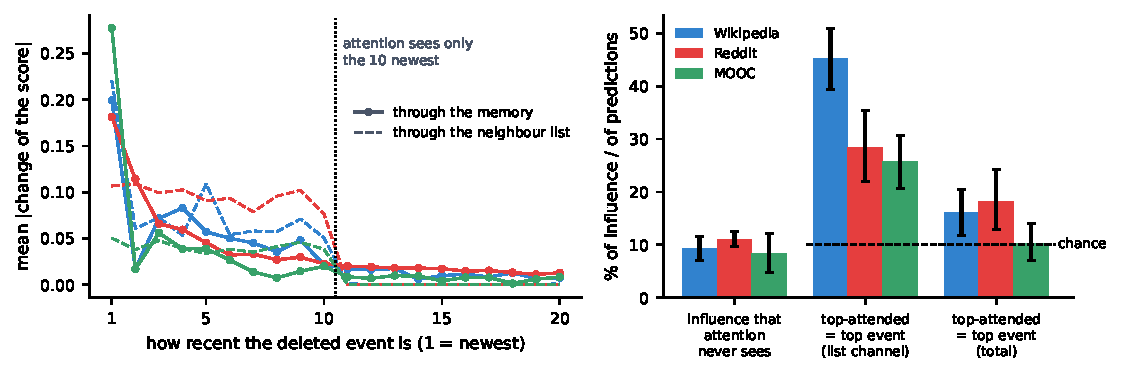
\includegraphics[width=\linewidth]{figures/influence.pdf}
\caption{Left: mean absolute change of a prediction's score when one of the user's past events is deleted, by how recent the
event is, through the memory and through the neighbour list. Right: share of the influence from events outside the 10 the
attention layer sees, and how often the most-attended event is the most influential one (95\% bootstrap intervals).}
\label{fig:infl}
\end{figure}

\end{document}
